\documentclass[conference]{IEEEtran}

\usepackage[T1]{fontenc}
\usepackage{newtxtext}
\usepackage{amsmath}
\usepackage{newtxmath}
\usepackage{icomma}
\usepackage{booktabs}
\usepackage{array}
\usepackage{graphicx}
\usepackage{cite}
\usepackage{xcolor}
\usepackage{tikz}
\usetikzlibrary{arrows.meta,positioning,shapes.geometric}
\usepackage[hyphens]{url}
\def\UrlBreaks{\do\/\do\.\do\-}

% Automatically generated by paper/scripts/gen_numbers.py from analysis_root/out_addendum2/*.csv,
% analysis_root/out_addendum3/*.csv, raw run outputs (queries.npz, epochs.parquet, summary.json,
% failed_runs.json, RUN_ADD3.log), repo/results/pilot/, and constants from audit/M3_DESIGN_CHECK.md.
% Do not edit by hand.
\newcommand{\RNumAddThreeChargedDCForcedSumBFourNewTopic}{$16$}
\newcommand{\RNumAddThreeCompRows}{$32$}
\newcommand{\RNumAddThreeDCUnspentEpochBytes}{$24,448$}
\newcommand{\RNumAddThreeMOneChargedDCRecentNewTopic}{$0.4809$}
\newcommand{\RNumAddThreeMOneChargedDCRecentSteady}{$0.7020$}
\newcommand{\RNumAddThreeMOneRuns}{$10$}
\newcommand{\RNumAddThreeMThreeChargedDCRecentBEightNewTopic}{$0.3179$}
\newcommand{\RNumAddThreeMThreeChargedDCRecentBEightSteady}{$0.3374$}
\newcommand{\RNumAddThreeMThreeChargedDCRecentBFourNewTopic}{$0.3041$}
\newcommand{\RNumAddThreeMThreeChargedDCRecentBFourSteady}{$0.3312$}
\newcommand{\RNumAddThreeMThreeChargedDCRecentBTwoNewTopic}{$0.2726$}
\newcommand{\RNumAddThreeMThreeChargedDCRecentBTwoSteady}{$0.3313$}
\newcommand{\RNumAddThreeMThreeFailedAttempts}{$22$}
\newcommand{\RNumAddThreeMThreeRuns}{$30$}
\newcommand{\RNumAddThreePOneBound}{$-1.00$~pp}
\newcommand{\RNumAddThreePTwoBound}{$0.00$~pp}
\newcommand{\RNumAddThreeRNExtraEpochBytesVsChargedDC}{$21,504$}
\newcommand{\RNumAddThreeRNForcedSumBFourNewTopic}{$100$}
\newcommand{\RNumAddThreeRNMinusUnchargedDCBTwoNewTopicAbsMean}{$2.11$~pp}
\newcommand{\RNumAddThreeRepRuns}{$2$}
\newcommand{\RNumAddThreeTotalIntervals}{$64$}
\newcommand{\RNumAddThreeTotalRefreshesBFour}{$750$}
\newcommand{\RNumAddThreeTotalRuns}{$42$}
\newcommand{\RNumAddThreeXFourDCNewTopic}{$-0.63$~pp $[-0.89,$ $-0.38]$}
\newcommand{\RNumAddThreeXFourDCNewTopicAbsMean}{$0.63$~pp}
\newcommand{\RNumAddThreeXFourDCNewTopicBootLow}{$-0.89$~pp}
\newcommand{\RNumAddThreeXFourDCNewTopicCell}{$-0.63$ $[-0.89,$ $-0.38]$}
\newcommand{\RNumAddThreeXFourDCNewTopicMean}{$-0.63$~pp}
\newcommand{\RNumAddThreeXFourDCNewTopicTInt}{$[-0.85,$ $-0.42]$~pp}
\newcommand{\RNumAddThreeXFourDCOverallNewTopic}{$-0.06$~pp $[-0.14,$ $+0.01]$}
\newcommand{\RNumAddThreeXFourDCOverallSteady}{$+0.04$~pp $[+0.01,$ $+0.08]$}
\newcommand{\RNumAddThreeXFourDCSteady}{$+0.17$~pp $[-0.01,$ $+0.35]$}
\newcommand{\RNumAddThreeXFourDCSteadyAbsMean}{$0.17$~pp}
\newcommand{\RNumAddThreeXFourDCSteadyBootLow}{$-0.01$~pp}
\newcommand{\RNumAddThreeXFourDCSteadyCell}{$+0.17$ $[-0.01,$ $+0.35]$}
\newcommand{\RNumAddThreeXFourDCSteadyMean}{$+0.17$~pp}
\newcommand{\RNumAddThreeXFourDCSteadyTInt}{$[-0.06,$ $+0.41]$~pp}
\newcommand{\RNumAddThreeXFourESNewTopic}{$+0.38$~pp $[+0.01,$ $+0.74]$}
\newcommand{\RNumAddThreeXFourESNewTopicAbsMean}{$0.38$~pp}
\newcommand{\RNumAddThreeXFourESNewTopicBootLow}{$+0.01$~pp}
\newcommand{\RNumAddThreeXFourESNewTopicCell}{$+0.38$ $[+0.01,$ $+0.74]$}
\newcommand{\RNumAddThreeXFourESNewTopicEarlyMean}{$+0.68$~pp}
\newcommand{\RNumAddThreeXFourESNewTopicLateMean}{$-0.20$~pp}
\newcommand{\RNumAddThreeXFourESNewTopicMean}{$+0.38$~pp}
\newcommand{\RNumAddThreeXFourESNewTopicTInt}{$[+0.13,$ $+0.64]$~pp}
\newcommand{\RNumAddThreeXFourESONewTopic}{$+0.43$~pp $[+0.07,$ $+0.79]$}
\newcommand{\RNumAddThreeXFourESONewTopicAbsMean}{$0.43$~pp}
\newcommand{\RNumAddThreeXFourESONewTopicBootLow}{$+0.07$~pp}
\newcommand{\RNumAddThreeXFourESONewTopicCell}{$+0.43$ $[+0.07,$ $+0.79]$}
\newcommand{\RNumAddThreeXFourESONewTopicMean}{$+0.43$~pp}
\newcommand{\RNumAddThreeXFourESONewTopicTInt}{$[+0.19,$ $+0.68]$~pp}
\newcommand{\RNumAddThreeXFourESOOverallNewTopic}{$-0.17$~pp $[-0.35,$ $+0.04]$}
\newcommand{\RNumAddThreeXFourESOOverallSteady}{$-0.71$~pp $[-0.95,$ $-0.53]$}
\newcommand{\RNumAddThreeXFourESOSteady}{$-0.45$~pp $[-0.75,$ $-0.12]$}
\newcommand{\RNumAddThreeXFourESOSteadyAbsMean}{$0.45$~pp}
\newcommand{\RNumAddThreeXFourESOSteadyBootLow}{$-0.75$~pp}
\newcommand{\RNumAddThreeXFourESOSteadyCell}{$-0.45$ $[-0.75,$ $-0.12]$}
\newcommand{\RNumAddThreeXFourESOSteadyMean}{$-0.45$~pp}
\newcommand{\RNumAddThreeXFourESOSteadyTInt}{$[-0.86,$ $-0.05]$~pp}
\newcommand{\RNumAddThreeXFourESOverallNewTopic}{$-0.20$~pp $[-0.38,$ $+0.02]$}
\newcommand{\RNumAddThreeXFourESOverallSteady}{$-0.74$~pp $[-0.98,$ $-0.55]$}
\newcommand{\RNumAddThreeXFourESSteady}{$-0.49$~pp $[-0.78,$ $-0.16]$}
\newcommand{\RNumAddThreeXFourESSteadyAbsMean}{$0.49$~pp}
\newcommand{\RNumAddThreeXFourESSteadyBootLow}{$-0.78$~pp}
\newcommand{\RNumAddThreeXFourESSteadyCell}{$-0.49$ $[-0.78,$ $-0.16]$}
\newcommand{\RNumAddThreeXFourESSteadyMean}{$-0.49$~pp}
\newcommand{\RNumAddThreeXFourESSteadyTInt}{$[-0.90,$ $-0.08]$~pp}
\newcommand{\RNumAddThreeXFourPVNewTopic}{$-2.39$~pp $[-2.84,$ $-1.99]$}
\newcommand{\RNumAddThreeXFourPVNewTopicAbsMean}{$2.39$~pp}
\newcommand{\RNumAddThreeXFourPVNewTopicBootLow}{$-2.84$~pp}
\newcommand{\RNumAddThreeXFourPVNewTopicCell}{$-2.39$ $[-2.84,$ $-1.99]$}
\newcommand{\RNumAddThreeXFourPVNewTopicMean}{$-2.39$~pp}
\newcommand{\RNumAddThreeXFourPVNewTopicTInt}{$[-2.73,$ $-2.08]$~pp}
\newcommand{\RNumAddThreeXFourPVOverallNewTopic}{$-0.40$~pp $[-0.56,$ $-0.21]$}
\newcommand{\RNumAddThreeXFourPVOverallSteady}{$-0.47$~pp $[-0.70,$ $-0.26]$}
\newcommand{\RNumAddThreeXFourPVSteady}{$-1.54$~pp $[-1.96,$ $-1.12]$}
\newcommand{\RNumAddThreeXFourPVSteadyAbsMean}{$1.54$~pp}
\newcommand{\RNumAddThreeXFourPVSteadyBootLow}{$-1.96$~pp}
\newcommand{\RNumAddThreeXFourPVSteadyCell}{$-1.54$ $[-1.96,$ $-1.12]$}
\newcommand{\RNumAddThreeXFourPVSteadyMean}{$-1.54$~pp}
\newcommand{\RNumAddThreeXFourPVSteadyTInt}{$[-2.12,$ $-0.96]$~pp}
\newcommand{\RNumAddThreeXOneAllZeroGapBFourNewTopic}{$+5.42$~pp}
\newcommand{\RNumAddThreeXOneAllZeroQueriesBFourNewTopic}{$1,428$}
\newcommand{\RNumAddThreeXOneChoiceShareBFour}{$74\%$}
\newcommand{\RNumAddThreeXOneNonZeroGapBFourNewTopic}{$+1.86$~pp}
\newcommand{\RNumAddThreeXOneNonZeroQueriesBFourNewTopic}{$4,947$}
\newcommand{\RNumAddThreeXOnePosSeedsBFourBEight}{$10$}
\newcommand{\RNumAddThreeXOneRNBEightNewTopic}{$+1.76$~pp $[+1.04,$ $+2.59]$}
\newcommand{\RNumAddThreeXOneRNBEightNewTopicAbsMean}{$1.76$~pp}
\newcommand{\RNumAddThreeXOneRNBEightNewTopicCell}{$+1.76$ $[+1.04,$ $+2.59]$}
\newcommand{\RNumAddThreeXOneRNBEightNewTopicMean}{$+1.76$~pp}
\newcommand{\RNumAddThreeXOneRNBEightNewTopicTInt}{$[+0.73,$ $+2.79]$~pp}
\newcommand{\RNumAddThreeXOneRNBEightSteady}{$+0.19$~pp $[-0.29,$ $+0.64]$}
\newcommand{\RNumAddThreeXOneRNBEightSteadyAbsMean}{$0.19$~pp}
\newcommand{\RNumAddThreeXOneRNBEightSteadyCell}{$+0.19$ $[-0.29,$ $+0.64]$}
\newcommand{\RNumAddThreeXOneRNBEightSteadyMean}{$+0.19$~pp}
\newcommand{\RNumAddThreeXOneRNBEightSteadyTInt}{$[-0.46,$ $+0.83]$~pp}
\newcommand{\RNumAddThreeXOneRNBFourNewTopic}{$+2.66$~pp $[+1.46,$ $+4.00]$}
\newcommand{\RNumAddThreeXOneRNBFourNewTopicAbsMean}{$2.66$~pp}
\newcommand{\RNumAddThreeXOneRNBFourNewTopicCell}{$+2.66$ $[+1.46,$ $+4.00]$}
\newcommand{\RNumAddThreeXOneRNBFourNewTopicMean}{$+2.66$~pp}
\newcommand{\RNumAddThreeXOneRNBFourNewTopicTInt}{$[+0.91,$ $+4.57]$~pp}
\newcommand{\RNumAddThreeXOneRNBFourSteady}{$+0.19$~pp $[-0.29,$ $+0.63]$}
\newcommand{\RNumAddThreeXOneRNBFourSteadyAbsMean}{$0.19$~pp}
\newcommand{\RNumAddThreeXOneRNBFourSteadyCell}{$+0.19$ $[-0.29,$ $+0.63]$}
\newcommand{\RNumAddThreeXOneRNBFourSteadyMean}{$+0.19$~pp}
\newcommand{\RNumAddThreeXOneRNBFourSteadyTInt}{$[-0.26,$ $+0.64]$~pp}
\newcommand{\RNumAddThreeXOneRNBTwoNewTopic}{$+0.48$~pp $[-0.48,$ $+1.66]$}
\newcommand{\RNumAddThreeXOneRNBTwoNewTopicAbsMean}{$0.48$~pp}
\newcommand{\RNumAddThreeXOneRNBTwoNewTopicCell}{$+0.48$ $[-0.48,$ $+1.66]$}
\newcommand{\RNumAddThreeXOneRNBTwoNewTopicMean}{$+0.48$~pp}
\newcommand{\RNumAddThreeXOneRNBTwoNewTopicTInt}{$[-0.88,$ $+1.95]$~pp}
\newcommand{\RNumAddThreeXOneRNBTwoSteady}{$+0.30$~pp $[-0.29,$ $+0.88]$}
\newcommand{\RNumAddThreeXOneRNBTwoSteadyAbsMean}{$0.30$~pp}
\newcommand{\RNumAddThreeXOneRNBTwoSteadyCell}{$+0.30$ $[-0.29,$ $+0.88]$}
\newcommand{\RNumAddThreeXOneRNBTwoSteadyMean}{$+0.30$~pp}
\newcommand{\RNumAddThreeXOneRNBTwoSteadyTInt}{$[-0.44,$ $+1.05]$~pp}
\newcommand{\RNumAddThreeXOneRNOverallBEightNewTopic}{$+0.12$~pp $[+0.03,$ $+0.22]$}
\newcommand{\RNumAddThreeXOneRNOverallBEightSteady}{$-0.05$~pp $[-0.15,$ $+0.06]$}
\newcommand{\RNumAddThreeXOneRNOverallBFourNewTopic}{$+0.42$~pp $[+0.11,$ $+0.69]$}
\newcommand{\RNumAddThreeXOneRNOverallBFourSteady}{$-0.12$~pp $[-0.26,$ $+0.00]$}
\newcommand{\RNumAddThreeXOneRNOverallBTwoNewTopic}{$+0.61$~pp $[+0.26,$ $+0.98]$}
\newcommand{\RNumAddThreeXOneRNOverallBTwoSteady}{$-0.04$~pp $[-0.18,$ $+0.11]$}
\newcommand{\RNumAddThreeXThreeDCBEightNewTopic}{$+0.16$~pp $[-0.10,$ $+0.41]$}
\newcommand{\RNumAddThreeXThreeDCBEightNewTopicAbsMean}{$0.16$~pp}
\newcommand{\RNumAddThreeXThreeDCBEightNewTopicCell}{$+0.16$ $[-0.10,$ $+0.41]$}
\newcommand{\RNumAddThreeXThreeDCBEightNewTopicMean}{$+0.16$~pp}
\newcommand{\RNumAddThreeXThreeDCBEightSteady}{$+0.00$~pp $[-0.17,$ $+0.19]$}
\newcommand{\RNumAddThreeXThreeDCBEightSteadyAbsMean}{$0.00$~pp}
\newcommand{\RNumAddThreeXThreeDCBEightSteadyCell}{$+0.00$ $[-0.17,$ $+0.19]$}
\newcommand{\RNumAddThreeXThreeDCBEightSteadyMean}{$+0.00$~pp}
\newcommand{\RNumAddThreeXThreeDCBFourNewTopic}{$-0.94$~pp $[-1.55,$ $-0.32]$}
\newcommand{\RNumAddThreeXThreeDCBFourNewTopicAbsMean}{$0.94$~pp}
\newcommand{\RNumAddThreeXThreeDCBFourNewTopicCell}{$-0.94$ $[-1.55,$ $-0.32]$}
\newcommand{\RNumAddThreeXThreeDCBFourNewTopicMean}{$-0.94$~pp}
\newcommand{\RNumAddThreeXThreeDCBFourSteady}{$-0.20$~pp $[-0.71,$ $+0.30]$}
\newcommand{\RNumAddThreeXThreeDCBFourSteadyAbsMean}{$0.20$~pp}
\newcommand{\RNumAddThreeXThreeDCBFourSteadyCell}{$-0.20$ $[-0.71,$ $+0.30]$}
\newcommand{\RNumAddThreeXThreeDCBFourSteadyMean}{$-0.20$~pp}
\newcommand{\RNumAddThreeXThreeDCBTwoNewTopic}{$-1.63$~pp $[-2.90,$ $-0.48]$}
\newcommand{\RNumAddThreeXThreeDCBTwoNewTopicAbsMean}{$1.63$~pp}
\newcommand{\RNumAddThreeXThreeDCBTwoNewTopicCell}{$-1.63$ $[-2.90,$ $-0.48]$}
\newcommand{\RNumAddThreeXThreeDCBTwoNewTopicMean}{$-1.63$~pp}
\newcommand{\RNumAddThreeXThreeDCBTwoSteady}{$+0.33$~pp $[-0.39,$ $+1.08]$}
\newcommand{\RNumAddThreeXThreeDCBTwoSteadyAbsMean}{$0.33$~pp}
\newcommand{\RNumAddThreeXThreeDCBTwoSteadyCell}{$+0.33$ $[-0.39,$ $+1.08]$}
\newcommand{\RNumAddThreeXThreeDCBTwoSteadyMean}{$+0.33$~pp}
\newcommand{\RNumAddThreeXTwoESOBEightNewTopic}{$+1.63$~pp $[+0.27,$ $+2.95]$}
\newcommand{\RNumAddThreeXTwoESOBEightNewTopicAbsMean}{$1.63$~pp}
\newcommand{\RNumAddThreeXTwoESOBEightNewTopicCell}{$+1.63$ $[+0.27,$ $+2.95]$}
\newcommand{\RNumAddThreeXTwoESOBEightNewTopicMean}{$+1.63$~pp}
\newcommand{\RNumAddThreeXTwoESOBEightNewTopicNegSeed}{$42$}
\newcommand{\RNumAddThreeXTwoESOBEightNewTopicNegSeedGap}{$-0.17$~pp}
\newcommand{\RNumAddThreeXTwoESOBEightNewTopicTInt}{$[+0.10,$ $+3.17]$~pp}
\newcommand{\RNumAddThreeXTwoESOBEightSteady}{$-4.28$~pp $[-5.17,$ $-3.42]$}
\newcommand{\RNumAddThreeXTwoESOBEightSteadyAbsMean}{$4.28$~pp}
\newcommand{\RNumAddThreeXTwoESOBEightSteadyCell}{$-4.28$ $[-5.17,$ $-3.42]$}
\newcommand{\RNumAddThreeXTwoESOBEightSteadyMean}{$-4.28$~pp}
\newcommand{\RNumAddThreeXTwoESOBEightSteadyTInt}{$[-5.31,$ $-3.25]$~pp}
\newcommand{\RNumAddThreeXTwoESOBFourNewTopic}{$+2.92$~pp $[+1.39,$ $+4.26]$}
\newcommand{\RNumAddThreeXTwoESOBFourNewTopicAbsMean}{$2.92$~pp}
\newcommand{\RNumAddThreeXTwoESOBFourNewTopicCell}{$+2.92$ $[+1.39,$ $+4.26]$}
\newcommand{\RNumAddThreeXTwoESOBFourNewTopicMean}{$+2.92$~pp}
\newcommand{\RNumAddThreeXTwoESOBFourNewTopicTInt}{$[+1.11,$ $+4.81]$~pp}
\newcommand{\RNumAddThreeXTwoESOBFourSteady}{$-2.29$~pp $[-2.90,$ $-1.68]$}
\newcommand{\RNumAddThreeXTwoESOBFourSteadyAbsMean}{$2.29$~pp}
\newcommand{\RNumAddThreeXTwoESOBFourSteadyCell}{$-2.29$ $[-2.90,$ $-1.68]$}
\newcommand{\RNumAddThreeXTwoESOBFourSteadyMean}{$-2.29$~pp}
\newcommand{\RNumAddThreeXTwoESOBFourSteadyTInt}{$[-2.85,$ $-1.74]$~pp}
\newcommand{\RNumAddThreeXTwoESOBTwoNewTopic}{$+1.12$~pp $[-0.39,$ $+2.62]$}
\newcommand{\RNumAddThreeXTwoESOBTwoNewTopicAbsMean}{$1.12$~pp}
\newcommand{\RNumAddThreeXTwoESOBTwoNewTopicCell}{$+1.12$ $[-0.39,$ $+2.62]$}
\newcommand{\RNumAddThreeXTwoESOBTwoNewTopicMean}{$+1.12$~pp}
\newcommand{\RNumAddThreeXTwoESOBTwoNewTopicTInt}{$[-0.90,$ $+3.15]$~pp}
\newcommand{\RNumAddThreeXTwoESOBTwoSteady}{$-0.87$~pp $[-1.41,$ $-0.36]$}
\newcommand{\RNumAddThreeXTwoESOBTwoSteadyAbsMean}{$0.87$~pp}
\newcommand{\RNumAddThreeXTwoESOBTwoSteadyCell}{$-0.87$ $[-1.41,$ $-0.36]$}
\newcommand{\RNumAddThreeXTwoESOBTwoSteadyMean}{$-0.87$~pp}
\newcommand{\RNumAddThreeXTwoESOBTwoSteadyTInt}{$[-1.40,$ $-0.33]$~pp}
\newcommand{\RNumAddThreeXTwoESOOverallBEightNewTopic}{$-3.43$~pp $[-3.77,$ $-3.02]$}
\newcommand{\RNumAddThreeXTwoESOOverallBEightSteady}{$-6.20$~pp $[-6.32,$ $-6.07]$}
\newcommand{\RNumAddThreeXTwoESOOverallBFourNewTopic}{$-0.79$~pp $[-1.26,$ $-0.25]$}
\newcommand{\RNumAddThreeXTwoESOOverallBFourSteady}{$-3.63$~pp $[-3.81,$ $-3.46]$}
\newcommand{\RNumAddThreeXTwoESOOverallBTwoNewTopic}{$+0.10$~pp $[-0.19,$ $+0.37]$}
\newcommand{\RNumAddThreeXTwoESOOverallBTwoSteady}{$-1.77$~pp $[-1.89,$ $-1.63]$}
\newcommand{\RNumAddThreeXTwoPVBEightNewTopic}{$-3.42$~pp $[-5.15,$ $-1.75]$}
\newcommand{\RNumAddThreeXTwoPVBEightNewTopicAbsMean}{$3.42$~pp}
\newcommand{\RNumAddThreeXTwoPVBEightNewTopicCell}{$-3.42$ $[-5.15,$ $-1.75]$}
\newcommand{\RNumAddThreeXTwoPVBEightNewTopicMean}{$-3.42$~pp}
\newcommand{\RNumAddThreeXTwoPVBEightNewTopicTInt}{$[-5.56,$ $-1.28]$~pp}
\newcommand{\RNumAddThreeXTwoPVBEightSteady}{$-7.16$~pp $[-7.98,$ $-6.33]$}
\newcommand{\RNumAddThreeXTwoPVBEightSteadyAbsMean}{$7.16$~pp}
\newcommand{\RNumAddThreeXTwoPVBEightSteadyCell}{$-7.16$ $[-7.98,$ $-6.33]$}
\newcommand{\RNumAddThreeXTwoPVBEightSteadyMean}{$-7.16$~pp}
\newcommand{\RNumAddThreeXTwoPVBEightSteadyTInt}{$[-7.99,$ $-6.36]$~pp}
\newcommand{\RNumAddThreeXTwoPVBFourNewTopic}{$+0.10$~pp $[-1.40,$ $+1.52]$}
\newcommand{\RNumAddThreeXTwoPVBFourNewTopicAbsMean}{$0.10$~pp}
\newcommand{\RNumAddThreeXTwoPVBFourNewTopicCell}{$+0.10$ $[-1.40,$ $+1.52]$}
\newcommand{\RNumAddThreeXTwoPVBFourNewTopicMean}{$+0.10$~pp}
\newcommand{\RNumAddThreeXTwoPVBFourNewTopicTInt}{$[-1.70,$ $+1.96]$~pp}
\newcommand{\RNumAddThreeXTwoPVBFourSteady}{$-3.87$~pp $[-4.72,$ $-3.11]$}
\newcommand{\RNumAddThreeXTwoPVBFourSteadyAbsMean}{$3.87$~pp}
\newcommand{\RNumAddThreeXTwoPVBFourSteadyCell}{$-3.87$ $[-4.72,$ $-3.11]$}
\newcommand{\RNumAddThreeXTwoPVBFourSteadyMean}{$-3.87$~pp}
\newcommand{\RNumAddThreeXTwoPVBFourSteadyTInt}{$[-4.76,$ $-3.00]$~pp}
\newcommand{\RNumAddThreeXTwoPVBTwoNewTopic}{$-0.16$~pp $[-1.89,$ $+1.49]$}
\newcommand{\RNumAddThreeXTwoPVBTwoNewTopicAbsMean}{$0.16$~pp}
\newcommand{\RNumAddThreeXTwoPVBTwoNewTopicCell}{$-0.16$ $[-1.89,$ $+1.49]$}
\newcommand{\RNumAddThreeXTwoPVBTwoNewTopicMean}{$-0.16$~pp}
\newcommand{\RNumAddThreeXTwoPVBTwoNewTopicTInt}{$[-2.56,$ $+2.18]$~pp}
\newcommand{\RNumAddThreeXTwoPVBTwoSteady}{$-1.58$~pp $[-2.11,$ $-1.06]$}
\newcommand{\RNumAddThreeXTwoPVBTwoSteadyAbsMean}{$1.58$~pp}
\newcommand{\RNumAddThreeXTwoPVBTwoSteadyCell}{$-1.58$ $[-2.11,$ $-1.06]$}
\newcommand{\RNumAddThreeXTwoPVBTwoSteadyMean}{$-1.58$~pp}
\newcommand{\RNumAddThreeXTwoPVBTwoSteadyTInt}{$[-1.97,$ $-1.19]$~pp}
\newcommand{\RNumAddThreeXTwoPVOverallBEightNewTopic}{$-1.12$~pp $[-1.60,$ $-0.64]$}
\newcommand{\RNumAddThreeXTwoPVOverallBEightSteady}{$-3.68$~pp $[-3.82,$ $-3.52]$}
\newcommand{\RNumAddThreeXTwoPVOverallBFourNewTopic}{$+0.33$~pp $[-0.26,$ $+0.93]$}
\newcommand{\RNumAddThreeXTwoPVOverallBFourSteady}{$-2.11$~pp $[-2.29,$ $-1.93]$}
\newcommand{\RNumAddThreeXTwoPVOverallBTwoNewTopic}{$+0.62$~pp $[+0.35,$ $+0.90]$}
\newcommand{\RNumAddThreeXTwoPVOverallBTwoSteady}{$-1.07$~pp $[-1.23,$ $-0.89]$}
\newcommand{\RNumAddendumTwoMTwoDone}{$140/330$}
\newcommand{\RNumAlwaysFreshEpochBytes}{$786,432$}
\newcommand{\RNumBootNarrowerMax}{$27\%$}
\newcommand{\RNumBootNarrowerMin}{$19\%$}
\newcommand{\RNumBootSeed}{$42$}
\newcommand{\RNumBootWiderMThreeRNMinusQLNewTopic}{$51\%$}
\newcommand{\RNumBudgetBFourEpochBytes}{$98,304$}
\newcommand{\RNumCIPct}{$95\%$}
\newcommand{\RNumCentersPerSummary}{$16$}
\newcommand{\RNumChanceRecallMTwo}{$0.0625$}
\newcommand{\RNumCorpusTotalPassages}{$100,000$}
\newcommand{\RNumDCScoreEpochBytes}{$128$}
\newcommand{\RNumDataSeed}{$42$}
\newcommand{\RNumESLoadPctBEight}{$29.5\%$}
\newcommand{\RNumESLoadPctBFour}{$14.8\%$}
\newcommand{\RNumESLoadPctBTwo}{$7.2\%$}
\newcommand{\RNumESLoadPctQEightHundred}{$3.7\%$}
\newcommand{\RNumESLoadPctQFifty}{$59.0\%$}
\newcommand{\RNumESLoadPctQTwoHundred}{$14.8\%$}
\newcommand{\RNumESOQFiftyMaxSearches}{$50$}
\newcommand{\RNumESOUnderspendVsESQFiftyBytes}{$14,904$}
\newcommand{\RNumESOUnspentMinBytesQFifty}{$15,504$}
\newcommand{\RNumESQFiftySecondShardSearches}{$9$}
\newcommand{\RNumEpochsPerCondition}{$250$}
\newcommand{\RNumExtraSearchesBFour}{$59$}
\newcommand{\RNumFiveSeeds}{$5$}
\newcommand{\RNumForcedShareDCNewTopicMOne}{$6.9\%$}
\newcommand{\RNumForcedShareDCNewTopicMThree}{$2.4\%$}
\newcommand{\RNumForcedShareDCSteadyMOne}{$0.0\%$}
\newcommand{\RNumForcedShareDCSteadyMThree}{$0.0\%$}
\newcommand{\RNumForcedShareQLNewTopicMOne}{$27.3\%$}
\newcommand{\RNumForcedShareQLNewTopicMThree}{$17.1\%$}
\newcommand{\RNumForcedShareQLSteadyMOne}{$27.9\%$}
\newcommand{\RNumForcedShareQLSteadyMThree}{$17.7\%$}
\newcommand{\RNumForcedShareRNNewTopicMOne}{$21.7\%$}
\newcommand{\RNumForcedShareRNNewTopicMOneQEightHundred}{$21.7\%$}
\newcommand{\RNumForcedShareRNNewTopicMOneQFifty}{$21.7\%$}
\newcommand{\RNumForcedShareRNNewTopicMOneQTwoHundred}{$21.7\%$}
\newcommand{\RNumForcedShareRNNewTopicMThree}{$13.3\%$}
\newcommand{\RNumForcedShareRNNewTopicMThreeBEight}{$5.3\%$}
\newcommand{\RNumForcedShareRNNewTopicMThreeBFour}{$13.3\%$}
\newcommand{\RNumForcedShareRNNewTopicMThreeBTwo}{$0.0\%$}
\newcommand{\RNumForcedShareRNSteadyMOne}{$27.2\%$}
\newcommand{\RNumForcedShareRNSteadyMOneQEightHundred}{$27.2\%$}
\newcommand{\RNumForcedShareRNSteadyMOneQFifty}{$27.2\%$}
\newcommand{\RNumForcedShareRNSteadyMOneQTwoHundred}{$27.2\%$}
\newcommand{\RNumForcedShareRNSteadyMThree}{$17.2\%$}
\newcommand{\RNumForcedShareRNSteadyMThreeBEight}{$5.0\%$}
\newcommand{\RNumForcedShareRNSteadyMThreeBFour}{$17.2\%$}
\newcommand{\RNumForcedShareRNSteadyMThreeBTwo}{$0.0\%$}
\newcommand{\RNumForcedShareSSNewTopicMOne}{$26.9\%$}
\newcommand{\RNumForcedShareSSNewTopicMThree}{$18.0\%$}
\newcommand{\RNumForcedShareSSSteadyMOne}{$28.0\%$}
\newcommand{\RNumForcedShareSSSteadyMThree}{$17.1\%$}
\newcommand{\RNumFourRulesSummariesBFour}{$4$}
\newcommand{\RNumFourRulesSummariesBTwo}{$2$}
\newcommand{\RNumGateMThreeNewTopic}{$+6.74$~pp $[+5.16,$ $+8.16]$}
\newcommand{\RNumGateMThreeNewTopicMinSeed}{$42$}
\newcommand{\RNumGateMThreeNewTopicMinSeedGap}{$+4.10$~pp}
\newcommand{\RNumGateMThreeNewTopicTInt}{$[+4.79,$ $+8.75]$~pp}
\newcommand{\RNumGateMThreeNewTopicUnweightedMean}{$+6.77$~pp}
\newcommand{\RNumGateMThreeOverallNewTopic}{$+1.73$~pp $[+1.12,$ $+2.33]$}
\newcommand{\RNumGateMThreeOverallSteady}{$-0.91$~pp $[-1.02,$ $-0.79]$}
\newcommand{\RNumGateMThreeSteady}{$+1.16$~pp $[+0.38,$ $+1.91]$}
\newcommand{\RNumGateMTwoNewTopic}{$+22.61$~pp $[+20.83,$ $+24.40]$}
\newcommand{\RNumGateMTwoOverallNewTopic}{$+9.87$~pp $[+8.87,$ $+10.77]$}
\newcommand{\RNumGateMTwoOverallSteady}{$-1.59$~pp $[-1.74,$ $-1.45]$}
\newcommand{\RNumGateMTwoSteady}{$+1.66$~pp $[+1.17,$ $+2.24]$}
\newcommand{\RNumGateThresholdPP}{$5$~pp}
\newcommand{\RNumHFourBDCMinusPVBTwoNewTopicNegSeed}{$42$}
\newcommand{\RNumHFourBDCMinusPVBTwoNewTopicNegSeedGap}{$-0.29$~pp}
\newcommand{\RNumHFourBDCMinusPVBTwoNewTopicTInt}{$[-0.35,$ $+3.25]$~pp}
\newcommand{\RNumHFourBESOMinusPVBEightNewTopic}{$-5.05$~pp $[-6.47,$ $-3.79]$}
\newcommand{\RNumHFourBESOMinusPVBEightNewTopicCell}{$-5.05$ $[-6.47,$ $-3.79]$}
\newcommand{\RNumHFourBESOMinusPVBEightSteady}{$-2.89$~pp $[-3.79,$ $-2.05]$}
\newcommand{\RNumHFourBESOMinusPVBEightSteadyCell}{$-2.89$ $[-3.79,$ $-2.05]$}
\newcommand{\RNumHFourBESOMinusPVBFourNewTopic}{$-2.82$~pp $[-3.79,$ $-1.93]$}
\newcommand{\RNumHFourBESOMinusPVBFourNewTopicCell}{$-2.82$ $[-3.79,$ $-1.93]$}
\newcommand{\RNumHFourBESOMinusPVBFourSteady}{$-1.58$~pp $[-2.24,$ $-0.91]$}
\newcommand{\RNumHFourBESOMinusPVBFourSteadyCell}{$-1.58$ $[-2.24,$ $-0.91]$}
\newcommand{\RNumHFourBESOMinusPVBTwoNewTopic}{$-1.28$~pp $[-2.26,$ $-0.43]$}
\newcommand{\RNumHFourBESOMinusPVBTwoNewTopicCell}{$-1.28$ $[-2.26,$ $-0.43]$}
\newcommand{\RNumHFourBESOMinusPVBTwoSteady}{$-0.71$~pp $[-1.12,$ $-0.29]$}
\newcommand{\RNumHFourBESOMinusPVBTwoSteadyCell}{$-0.71$ $[-1.12,$ $-0.29]$}
\newcommand{\RNumHFourBRefMinusESOBEightNewTopic}{$+1.47$~pp $[+0.07,$ $+2.81]$}
\newcommand{\RNumHFourBRefMinusESOBEightNewTopicCell}{$+1.47$ $[+0.07,$ $+2.81]$}
\newcommand{\RNumHFourBRefMinusESOBEightNewTopicTInt}{$[-0.12,$ $+3.07]$~pp}
\newcommand{\RNumHFourBRefMinusESOBEightSteady}{$-4.28$~pp $[-5.17,$ $-3.43]$}
\newcommand{\RNumHFourBRefMinusESOBEightSteadyCell}{$-4.28$ $[-5.17,$ $-3.43]$}
\newcommand{\RNumHFourBRefMinusESOBFourNewTopic}{$+3.86$~pp $[+2.10,$ $+5.31]$}
\newcommand{\RNumHFourBRefMinusESOBFourNewTopicCell}{$+3.86$ $[+2.10,$ $+5.31]$}
\newcommand{\RNumHFourBRefMinusESOBFourSteady}{$-2.09$~pp $[-2.84,$ $-1.33]$}
\newcommand{\RNumHFourBRefMinusESOBFourSteadyCell}{$-2.09$ $[-2.84,$ $-1.33]$}
\newcommand{\RNumHFourBRefMinusESOBTwoNewTopic}{$+2.75$~pp $[+0.97,$ $+4.33]$}
\newcommand{\RNumHFourBRefMinusESOBTwoNewTopicCell}{$+2.75$ $[+0.97,$ $+4.33]$}
\newcommand{\RNumHFourBRefMinusESOBTwoSteady}{$-1.08$~pp $[-1.54,$ $-0.62]$}
\newcommand{\RNumHFourBRefMinusESOBTwoSteadyCell}{$-1.08$ $[-1.54,$ $-0.62]$}
\newcommand{\RNumHFourBRefMinusPVBEightNewTopic}{$-3.59$~pp $[-5.37,$ $-1.86]$}
\newcommand{\RNumHFourBRefMinusPVBEightNewTopicCell}{$-3.59$ $[-5.37,$ $-1.86]$}
\newcommand{\RNumHFourBRefMinusPVBEightSteady}{$-7.17$~pp $[-8.00,$ $-6.31]$}
\newcommand{\RNumHFourBRefMinusPVBEightSteadyCell}{$-7.17$ $[-8.00,$ $-6.31]$}
\newcommand{\RNumHFourBRefMinusPVBFourNewTopic}{$+1.04$~pp $[-0.50,$ $+2.53]$}
\newcommand{\RNumHFourBRefMinusPVBFourNewTopicCell}{$+1.04$ $[-0.50,$ $+2.53]$}
\newcommand{\RNumHFourBRefMinusPVBFourSteady}{$-3.67$~pp $[-4.57,$ $-2.85]$}
\newcommand{\RNumHFourBRefMinusPVBFourSteadyCell}{$-3.67$ $[-4.57,$ $-2.85]$}
\newcommand{\RNumHFourBRefMinusPVBTwoNewTopic}{$+1.47$~pp $[+0.03,$ $+2.90]$}
\newcommand{\RNumHFourBRefMinusPVBTwoNewTopicCell}{$+1.47$ $[+0.03,$ $+2.90]$}
\newcommand{\RNumHFourBRefMinusPVBTwoNewTopicLow}{$+0.03$~pp}
\newcommand{\RNumHFourBRefMinusPVBTwoSteady}{$-1.79$~pp $[-2.38,$ $-1.20]$}
\newcommand{\RNumHFourBRefMinusPVBTwoSteadyCell}{$-1.79$ $[-2.38,$ $-1.20]$}
\newcommand{\RNumHFourBRefMinusPVOverallBEightNewTopic}{$-1.13$~pp $[-1.66,$ $-0.61]$}
\newcommand{\RNumHFourBRefMinusPVOverallBEightSteady}{$-3.69$~pp $[-3.82,$ $-3.55]$}
\newcommand{\RNumHFourBRefMinusPVOverallBFourNewTopic}{$+0.33$~pp $[-0.29,$ $+0.97]$}
\newcommand{\RNumHFourBRefMinusPVOverallBFourSteady}{$-2.18$~pp $[-2.35,$ $-2.02]$}
\newcommand{\RNumHFourBRefMinusPVOverallBTwoNewTopic}{$+1.03$~pp $[+0.63,$ $+1.43]$}
\newcommand{\RNumHFourBRefMinusPVOverallBTwoSteady}{$-0.99$~pp $[-1.19,$ $-0.77]$}
\newcommand{\RNumHFourESMinusPVBEightNewTopic}{$-10.69$~pp $[-11.76,$ $-9.67]$}
\newcommand{\RNumHFourESMinusPVBEightNewTopicCell}{$-10.69$ $[-11.76,$ $-9.67]$}
\newcommand{\RNumHFourESMinusPVBEightSteady}{$-10.13$~pp $[-10.80,$ $-9.47]$}
\newcommand{\RNumHFourESMinusPVBEightSteadyCell}{$-10.13$ $[-10.80,$ $-9.47]$}
\newcommand{\RNumHFourESMinusPVBFourNewTopic}{$-5.40$~pp $[-6.11,$ $-4.70]$}
\newcommand{\RNumHFourESMinusPVBFourNewTopicCell}{$-5.40$ $[-6.11,$ $-4.70]$}
\newcommand{\RNumHFourESMinusPVBFourSteady}{$-5.18$~pp $[-5.76,$ $-4.65]$}
\newcommand{\RNumHFourESMinusPVBFourSteadyCell}{$-5.18$ $[-5.76,$ $-4.65]$}
\newcommand{\RNumHFourESMinusPVBTwoNewTopic}{$-2.53$~pp $[-3.28,$ $-1.85]$}
\newcommand{\RNumHFourESMinusPVBTwoNewTopicCell}{$-2.53$ $[-3.28,$ $-1.85]$}
\newcommand{\RNumHFourESMinusPVBTwoSteady}{$-2.66$~pp $[-3.00,$ $-2.32]$}
\newcommand{\RNumHFourESMinusPVBTwoSteadyCell}{$-2.66$ $[-3.00,$ $-2.32]$}
\newcommand{\RNumHFourRefMinusESBEightNewTopic}{$+20.33$~pp $[+18.33,$ $+22.26]$}
\newcommand{\RNumHFourRefMinusESBEightNewTopicCell}{$+20.33$ $[+18.33,$ $+22.26]$}
\newcommand{\RNumHFourRefMinusESBEightSteady}{$-0.03$~pp $[-0.59,$ $+0.65]$}
\newcommand{\RNumHFourRefMinusESBEightSteadyCell}{$-0.03$ $[-0.59,$ $+0.65]$}
\newcommand{\RNumHFourRefMinusESBFourNewTopic}{$+21.44$~pp $[+19.59,$ $+23.22]$}
\newcommand{\RNumHFourRefMinusESBFourNewTopicCell}{$+21.44$ $[+19.59,$ $+23.22]$}
\newcommand{\RNumHFourRefMinusESBFourSteady}{$+0.87$~pp $[+0.33,$ $+1.46]$}
\newcommand{\RNumHFourRefMinusESBFourSteadyCell}{$+0.87$ $[+0.33,$ $+1.46]$}
\newcommand{\RNumHFourRefMinusESBTwoNewTopic}{$+21.93$~pp $[+20.16,$ $+23.62]$}
\newcommand{\RNumHFourRefMinusESBTwoNewTopicCell}{$+21.93$ $[+20.16,$ $+23.62]$}
\newcommand{\RNumHFourRefMinusESBTwoSteady}{$+1.26$~pp $[+0.79,$ $+1.76]$}
\newcommand{\RNumHFourRefMinusESBTwoSteadyCell}{$+1.26$ $[+0.79,$ $+1.76]$}
\newcommand{\RNumHFourRefMinusPVBEightNewTopic}{$+9.64$~pp $[+8.04,$ $+11.26]$}
\newcommand{\RNumHFourRefMinusPVBEightNewTopicCell}{$+9.64$ $[+8.04,$ $+11.26]$}
\newcommand{\RNumHFourRefMinusPVBEightSteady}{$-10.15$~pp $[-11.02,$ $-9.23]$}
\newcommand{\RNumHFourRefMinusPVBEightSteadyCell}{$-10.15$ $[-11.02,$ $-9.23]$}
\newcommand{\RNumHFourRefMinusPVBFourNewTopic}{$+16.04$~pp $[+14.40,$ $+17.73]$}
\newcommand{\RNumHFourRefMinusPVBFourNewTopicCell}{$+16.04$ $[+14.40,$ $+17.73]$}
\newcommand{\RNumHFourRefMinusPVBFourSteady}{$-4.31$~pp $[-5.09,$ $-3.47]$}
\newcommand{\RNumHFourRefMinusPVBFourSteadyCell}{$-4.31$ $[-5.09,$ $-3.47]$}
\newcommand{\RNumHFourRefMinusPVBTwoNewTopic}{$+19.40$~pp $[+17.67,$ $+21.12]$}
\newcommand{\RNumHFourRefMinusPVBTwoNewTopicCell}{$+19.40$ $[+17.67,$ $+21.12]$}
\newcommand{\RNumHFourRefMinusPVBTwoSteady}{$-1.40$~pp $[-1.96,$ $-0.82]$}
\newcommand{\RNumHFourRefMinusPVBTwoSteadyCell}{$-1.40$ $[-1.96,$ $-0.82]$}
\newcommand{\RNumHFourRefMinusPVOverallBEightNewTopic}{$+6.12$~pp $[+5.14,$ $+7.02]$}
\newcommand{\RNumHFourRefMinusPVOverallBEightSteady}{$-5.38$~pp $[-5.59,$ $-5.19]$}
\newcommand{\RNumHFourRefMinusPVOverallBFourNewTopic}{$+8.04$~pp $[+7.04,$ $+8.96]$}
\newcommand{\RNumHFourRefMinusPVOverallBFourSteady}{$-3.44$~pp $[-3.65,$ $-3.26]$}
\newcommand{\RNumHFourRefMinusPVOverallBTwoNewTopic}{$+8.97$~pp $[+8.02,$ $+9.85]$}
\newcommand{\RNumHFourRefMinusPVOverallBTwoSteady}{$-2.53$~pp $[-2.68,$ $-2.38]$}
\newcommand{\RNumHOneGapNewTopic}{$+2.29$~pp $[+1.47,$ $+3.17]$}
\newcommand{\RNumHOneGapSteady}{$+0.55$~pp $[-0.07,$ $+1.12]$}
\newcommand{\RNumHOneOutOfSampleMaxNewTopic}{$+3.18$~pp}
\newcommand{\RNumHOneOutOfSampleMaxSteady}{$+1.31$~pp}
\newcommand{\RNumHOneOutOfSampleMeanNewTopic}{$+2.37$~pp}
\newcommand{\RNumHOneOutOfSampleMeanSteady}{$+0.52$~pp}
\newcommand{\RNumHOneOutOfSampleMinNewTopic}{$+1.66$}
\newcommand{\RNumHOneOutOfSampleMinSteady}{$-0.47$}
\newcommand{\RNumHOneOutOfSampleUnweightedMeanNewTopic}{$+2.41$~pp}
\newcommand{\RNumHOneOutOfSampleUnweightedMeanSteady}{$+0.52$~pp}
\newcommand{\RNumHOneOverallGapNewTopic}{$+0.58$~pp $[+0.35,$ $+0.80]$}
\newcommand{\RNumHOneOverallGapSteady}{$+0.00$~pp $[-0.25,$ $+0.23]$}
\newcommand{\RNumHThreeBMThreeRNMinusQLNewTopicTInt}{$[+0.03,$ $+0.93]$~pp}
\newcommand{\RNumHThreeBRNMinusDCNewTopic}{$-3.60$~pp $[-4.93,$ $-2.26]$}
\newcommand{\RNumHThreeBRNMinusDCNewTopicAbsMean}{$3.60$~pp}
\newcommand{\RNumHThreeBRNMinusDCOverallNewTopic}{$-0.42$~pp $[-0.71,$ $-0.10]$}
\newcommand{\RNumHThreeBRNMinusDCOverallNewTopicTInt}{$[-0.90,$ $+0.07]$~pp}
\newcommand{\RNumHThreeBRNMinusDCOverallSteady}{$+0.19$~pp $[+0.08,$ $+0.29]$}
\newcommand{\RNumHThreeBRNMinusDCSteady}{$-0.39$~pp $[-1.06,$ $+0.32]$}
\newcommand{\RNumHThreeBRNMinusQLNewTopic}{$+0.50$~pp $[-0.22,$ $+1.14]$}
\newcommand{\RNumHThreeBRNMinusQLOverallNewTopic}{$-0.10$~pp $[-0.31,$ $+0.10]$}
\newcommand{\RNumHThreeBRNMinusQLOverallSteady}{$-0.02$~pp $[-0.14,$ $+0.09]$}
\newcommand{\RNumHThreeBRNMinusQLSteady}{$-0.14$~pp $[-0.83,$ $+0.54]$}
\newcommand{\RNumHThreeBRNMinusRRNewTopic}{$+2.38$~pp $[+1.27,$ $+3.34]$}
\newcommand{\RNumHThreeBRNMinusRROverallNewTopic}{$+0.01$~pp $[-0.19,$ $+0.23]$}
\newcommand{\RNumHThreeBRNMinusRROverallSteady}{$+0.12$~pp $[+0.01,$ $+0.26]$}
\newcommand{\RNumHThreeBRNMinusRRSteady}{$+0.32$~pp $[-0.18,$ $+0.83]$}
\newcommand{\RNumHThreeBRNMinusSSNewTopic}{$-0.48$~pp $[-1.79,$ $+0.62]$}
\newcommand{\RNumHThreeBRNMinusSSOverallNewTopic}{$-0.31$~pp $[-0.62,$ $+0.02]$}
\newcommand{\RNumHThreeBRNMinusSSOverallSteady}{$+0.03$~pp $[-0.09,$ $+0.14]$}
\newcommand{\RNumHThreeBRNMinusSSSteady}{$-0.05$~pp $[-0.80,$ $+0.73]$}
\newcommand{\RNumHThreeGapZero}{$+0.00$~pp $[+0.00,$ $+0.00]$}
\newcommand{\RNumHTwoBESOvsRefreshNewTopic}{$+1.84$~pp $[+0.58,$ $+3.01]$}
\newcommand{\RNumHTwoBESOvsRefreshOverallNewTopic}{$+2.08$~pp $[+1.91,$ $+2.25]$}
\newcommand{\RNumHTwoBESOvsRefreshOverallSteady}{$+2.86$~pp $[+2.66,$ $+3.03]$}
\newcommand{\RNumHTwoBESOvsRefreshSteady}{$+2.55$~pp $[+2.17,$ $+2.97]$}
\newcommand{\RNumHTwoESvsRefreshNewTopic}{$+1.97$~pp $[+0.74,$ $+3.15]$}
\newcommand{\RNumHTwoESvsRefreshOverallNewTopic}{$+2.25$~pp $[+2.09,$ $+2.41]$}
\newcommand{\RNumHTwoESvsRefreshOverallSteady}{$+3.03$~pp $[+2.83,$ $+3.19]$}
\newcommand{\RNumHTwoESvsRefreshSteady}{$+2.76$~pp $[+2.33,$ $+3.22]$}
\newcommand{\RNumHTwoPVvsRefreshNewTopic}{$+2.09$~pp $[+1.00,$ $+3.27]$}
\newcommand{\RNumHTwoPVvsRefreshOverallNewTopic}{$+0.32$~pp $[+0.12,$ $+0.53]$}
\newcommand{\RNumHTwoPVvsRefreshOverallSteady}{$+0.54$~pp $[+0.38,$ $+0.74]$}
\newcommand{\RNumHTwoPVvsRefreshSteady}{$+1.88$~pp $[+1.44,$ $+2.36]$}
\newcommand{\RNumKMeansIters}{$15$}
\newcommand{\RNumLookaheadMOneMaxQTwoHundred}{$0.21$~pp}
\newcommand{\RNumLookaheadMOneQEightHundredNewTopic}{$+0.05$~pp $[+0.01,$ $+0.09]$}
\newcommand{\RNumLookaheadMOneQEightHundredNewTopicCell}{$+0.05$ $[+0.01,$ $+0.09]$}
\newcommand{\RNumLookaheadMOneQEightHundredSteady}{$+0.03$~pp $[+0.00,$ $+0.06]$}
\newcommand{\RNumLookaheadMOneQEightHundredSteadyCell}{$+0.03$ $[+0.00,$ $+0.06]$}
\newcommand{\RNumLookaheadMOneQFiftyNewTopic}{$+1.99$~pp $[+1.12,$ $+3.01]$}
\newcommand{\RNumLookaheadMOneQFiftyNewTopicCell}{$+1.99$ $[+1.12,$ $+3.01]$}
\newcommand{\RNumLookaheadMOneQFiftySteady}{$+1.33$~pp $[+0.77,$ $+2.00]$}
\newcommand{\RNumLookaheadMOneQFiftySteadyCell}{$+1.33$ $[+0.77,$ $+2.00]$}
\newcommand{\RNumLookaheadMOneQTwoHundredNewTopic}{$+0.13$~pp $[-0.07,$ $+0.35]$}
\newcommand{\RNumLookaheadMOneQTwoHundredNewTopicCell}{$+0.13$ $[-0.07,$ $+0.35]$}
\newcommand{\RNumLookaheadMOneQTwoHundredSteady}{$+0.21$~pp $[+0.03,$ $+0.37]$}
\newcommand{\RNumLookaheadMOneQTwoHundredSteadyCell}{$+0.21$ $[+0.03,$ $+0.37]$}
\newcommand{\RNumLookaheadMOneQTwoHundredSteadyNegSeed}{$45$}
\newcommand{\RNumLookaheadMOneQTwoHundredSteadyNegSeedGap}{$-0.04$~pp}
\newcommand{\RNumLookaheadMOneQTwoHundredSteadyTInt}{$[-0.00,$ $+0.42]$~pp}
\newcommand{\RNumLookaheadMThreeBEightNewTopic}{$+0.28$~pp $[+0.09,$ $+0.48]$}
\newcommand{\RNumLookaheadMThreeBEightSteady}{$+0.18$~pp $[+0.03,$ $+0.33]$}
\newcommand{\RNumLookaheadMThreeBFourNewTopic}{$+0.30$~pp $[+0.08,$ $+0.52]$}
\newcommand{\RNumLookaheadMThreeBFourSteady}{$+0.16$~pp $[-0.01,$ $+0.32]$}
\newcommand{\RNumLookaheadMThreeBTwoNewTopic}{$+0.24$~pp $[+0.07,$ $+0.40]$}
\newcommand{\RNumLookaheadMThreeBTwoSteady}{$-0.01$~pp $[-0.11,$ $+0.10]$}
\newcommand{\RNumLookaheadMThreeMaxBFour}{$0.30$~pp}
\newcommand{\RNumMOneAFRecentNewTopic}{$0.4872$}
\newcommand{\RNumMOneAFRecentSteady}{$0.7081$}
\newcommand{\RNumMOneAFShareOfOracleNewTopic}{$13.5\%$}
\newcommand{\RNumMOneAFShareOfOracleSteady}{$5.6\%$}
\newcommand{\RNumMOneAllShardsRecentNewTopic}{$0.9968$}
\newcommand{\RNumMOneAllShardsRecentSteady}{$0.9985$}
\newcommand{\RNumMOneDCMinusESOQEightHundredSteady}{$-0.63$~pp $[-0.88,$ $-0.36]$}
\newcommand{\RNumMOneDCMinusPVQFiftySteady}{$-1.26$~pp $[-2.33,$ $-0.19]$}
\newcommand{\RNumMOneDCMinusRNQFiftySteady}{$+0.63$~pp $[+0.02,$ $+1.29]$}
\newcommand{\RNumMOneDCRecentMeanNewTopic}{$0.4813$}
\newcommand{\RNumMOneDCRecentMeanQEightHundredSteady}{$0.7003$}
\newcommand{\RNumMOneDCRecentMeanQFiftySteady}{$0.7226$}
\newcommand{\RNumMOneDCRecentMeanSteady}{$0.7040$}
\newcommand{\RNumMOneDCRecentNewTopic}{$0.4813$}
\newcommand{\RNumMOneDCRecentSteady}{$0.7040$}
\newcommand{\RNumMOneESBytes}{$4,885,200$}
\newcommand{\RNumMOneESOBytesNewTopic}{$4,604,342$}
\newcommand{\RNumMOneESOBytesSteady}{$4,649,386$}
\newcommand{\RNumMOneESORecentNewTopic}{$0.4996$}
\newcommand{\RNumMOneESORecentSteady}{$0.7297$}
\newcommand{\RNumMOneESOShareOfESQEightHundredNewTopic}{$96.9\%$}
\newcommand{\RNumMOneESOShareOfESQEightHundredSteady}{$96.8\%$}
\newcommand{\RNumMOneESOShareOfESQFiftyNewTopic}{$83.0\%$}
\newcommand{\RNumMOneESOShareOfESQFiftySteady}{$83.1\%$}
\newcommand{\RNumMOneESOShareOfESQTwoHundredNewTopic}{$94.3\%$}
\newcommand{\RNumMOneESOShareOfESQTwoHundredSteady}{$95.2\%$}
\newcommand{\RNumMOneESRecentMeanNewTopic}{$0.5009$}
\newcommand{\RNumMOneESRecentMeanSteady}{$0.7317$}
\newcommand{\RNumMOneESRecentNewTopic}{$0.5009$}
\newcommand{\RNumMOneESRecentSteady}{$0.7317$}
\newcommand{\RNumMOneFourRulesBytes}{$4,915,200$}
\newcommand{\RNumMOneNRRecentNewTopic}{$0.4643$}
\newcommand{\RNumMOneNRRecentSteady}{$0.7026$}
\newcommand{\RNumMOneOracleRecentNewTopic}{$0.6335$}
\newcommand{\RNumMOneOracleRecentSteady}{$0.7996$}
\newcommand{\RNumMOnePVBytes}{$4,863,600$}
\newcommand{\RNumMOnePVPredRecentSteady}{$0.7214$}
\newcommand{\RNumMOnePVPushedVecs}{$3,150$}
\newcommand{\RNumMOnePVRecentMeanNewTopic}{$0.5022$}
\newcommand{\RNumMOnePVRecentMeanSteady}{$0.7230$}
\newcommand{\RNumMOnePVRecentNewTopic}{$0.5022$}
\newcommand{\RNumMOnePVRecentSteady}{$0.7230$}
\newcommand{\RNumMOnePVShareFracSteady}{$0.0630$}
\newcommand{\RNumMOnePVShareSteady}{$6.30\%$}
\newcommand{\RNumMOneQLRecentMeanNewTopic}{$0.4661$}
\newcommand{\RNumMOneQLRecentMeanSteady}{$0.7025$}
\newcommand{\RNumMOneQLRecentNewTopic}{$0.4661$}
\newcommand{\RNumMOneQLRecentSteady}{$0.7025$}
\newcommand{\RNumMOneQSweepSteadyRuleSpanQEightHundred}{$0.06$~pp}
\newcommand{\RNumMOneRNAmortBytes}{$7,913,728$}
\newcommand{\RNumMOneRNBytes}{$4,768,000$}
\newcommand{\RNumMOneRNRecentMeanNewTopic}{$0.4729$}
\newcommand{\RNumMOneRNRecentMeanQEightHundredSteady}{$0.6996$}
\newcommand{\RNumMOneRNRecentMeanQFiftySteady}{$0.7163$}
\newcommand{\RNumMOneRNRecentMeanSteady}{$0.7042$}
\newcommand{\RNumMOneRNRecentNewTopic}{$0.4729$}
\newcommand{\RNumMOneRNRecentSteady}{$0.7042$}
\newcommand{\RNumMOneRRRecentMeanNewTopic}{$0.4645$}
\newcommand{\RNumMOneRRRecentMeanSteady}{$0.7008$}
\newcommand{\RNumMOneRRRecentNewTopic}{$0.4645$}
\newcommand{\RNumMOneRRRecentSteady}{$0.7008$}
\newcommand{\RNumMOneSSRecentMeanNewTopic}{$0.4661$}
\newcommand{\RNumMOneSSRecentMeanSteady}{$0.7030$}
\newcommand{\RNumMOneSSRecentNewTopic}{$0.4661$}
\newcommand{\RNumMOneSSRecentSteady}{$0.7030$}
\newcommand{\RNumMThreeAFRecentNewTopic}{$0.3163$}
\newcommand{\RNumMThreeAFRecentSteady}{$0.3374$}
\newcommand{\RNumMThreeActiveEpochsPerStream}{$250$}
\newcommand{\RNumMThreeActiveNewTopicAllEight}{$244$}
\newcommand{\RNumMThreeActiveNewTopicBelowEight}{$6$}
\newcommand{\RNumMThreeActiveNewTopicFiveShards}{$2$}
\newcommand{\RNumMThreeActiveNewTopicMean}{$7.96$}
\newcommand{\RNumMThreeActiveNewTopicMin}{$5$}
\newcommand{\RNumMThreeActiveNewTopicSevenShards}{$4$}
\newcommand{\RNumMThreeActiveSteadyAllEight}{$250$}
\newcommand{\RNumMThreeActiveSteadyBelowEight}{$0$}
\newcommand{\RNumMThreeActiveSteadyMean}{$8.00$}
\newcommand{\RNumMThreeActiveSteadyMin}{$8$}
\newcommand{\RNumMThreeActiveTotalAllEight}{$494$}
\newcommand{\RNumMThreeActiveTotalEpochs}{$500$}
\newcommand{\RNumMThreeAllShardsRecentNewTopic}{$0.9967$}
\newcommand{\RNumMThreeAllShardsRecentSteady}{$0.9982$}
\newcommand{\RNumMThreeDCRecentBEightNewTopic}{$0.3163$}
\newcommand{\RNumMThreeDCRecentBEightSteady}{$0.3374$}
\newcommand{\RNumMThreeDCRecentBFourNewTopic}{$0.3135$}
\newcommand{\RNumMThreeDCRecentBFourSteady}{$0.3333$}
\newcommand{\RNumMThreeDCRecentBTwoNewTopic}{$0.2889$}
\newcommand{\RNumMThreeDCRecentBTwoSteady}{$0.3280$}
\newcommand{\RNumMThreeESORecentBEightNewTopic}{$0.3016$}
\newcommand{\RNumMThreeESORecentBEightSteady}{$0.3802$}
\newcommand{\RNumMThreeESORecentBFourNewTopic}{$0.2749$}
\newcommand{\RNumMThreeESORecentBFourSteady}{$0.3542$}
\newcommand{\RNumMThreeESORecentBTwoNewTopic}{$0.2613$}
\newcommand{\RNumMThreeESORecentBTwoSteady}{$0.3400$}
\newcommand{\RNumMThreeESOShareOfESBEightNewTopic}{$96.8\%$}
\newcommand{\RNumMThreeESOShareOfESBEightSteady}{$96.5\%$}
\newcommand{\RNumMThreeESOShareOfESBFourNewTopic}{$94.3\%$}
\newcommand{\RNumMThreeESOShareOfESBFourSteady}{$95.2\%$}
\newcommand{\RNumMThreeESOShareOfESBTwoNewTopic}{$90.8\%$}
\newcommand{\RNumMThreeESOShareOfESBTwoSteady}{$91.6\%$}
\newcommand{\RNumMThreeESOShareOfESMax}{$96.8\%$}
\newcommand{\RNumMThreeESOShareOfESMin}{$90.8\%$}
\newcommand{\RNumMThreeESOShareOfRefreshBTwoNewTopic}{$88.7\%$}
\newcommand{\RNumMThreeESOShareOfRefreshBTwoSteady}{$89.5\%$}
\newcommand{\RNumMThreeESOUnderspendValMax}{$0.18$~pp}
\newcommand{\RNumMThreeESOUnderspendValMin}{$0.13$}
\newcommand{\RNumMThreeESRecentBEightNewTopic}{$0.3044$}
\newcommand{\RNumMThreeESRecentBEightSteady}{$0.3820$}
\newcommand{\RNumMThreeESRecentBFourNewTopic}{$0.2778$}
\newcommand{\RNumMThreeESRecentBFourSteady}{$0.3557$}
\newcommand{\RNumMThreeESRecentBTwoNewTopic}{$0.2637$}
\newcommand{\RNumMThreeESRecentBTwoSteady}{$0.3399$}
\newcommand{\RNumMThreeNRRecentNewTopic}{$0.2489$}
\newcommand{\RNumMThreeNRRecentSteady}{$0.3258$}
\newcommand{\RNumMThreeOracleRecentNewTopic}{$0.4863$}
\newcommand{\RNumMThreeOracleRecentSteady}{$0.5046$}
\newcommand{\RNumMThreePVNewTopicExcessMax}{$1.0$~pp}
\newcommand{\RNumMThreePVNewTopicExcessMin}{$0.2$}
\newcommand{\RNumMThreePVPredRecentBEightSteady}{$0.4114$}
\newcommand{\RNumMThreePVPredRecentBFourSteady}{$0.3683$}
\newcommand{\RNumMThreePVPredRecentBTwoSteady}{$0.3467$}
\newcommand{\RNumMThreePVRecentBEightNewTopic}{$0.3521$}
\newcommand{\RNumMThreePVRecentBEightSteady}{$0.4090$}
\newcommand{\RNumMThreePVRecentBFourNewTopic}{$0.3031$}
\newcommand{\RNumMThreePVRecentBFourSteady}{$0.3700$}
\newcommand{\RNumMThreePVRecentBTwoNewTopic}{$0.2742$}
\newcommand{\RNumMThreePVRecentBTwoSteady}{$0.3471$}
\newcommand{\RNumMThreeQLRecentBEightNewTopic}{$0.3163$}
\newcommand{\RNumMThreeQLRecentBEightSteady}{$0.3374$}
\newcommand{\RNumMThreeQLRecentBFourNewTopic}{$0.2726$}
\newcommand{\RNumMThreeQLRecentBFourSteady}{$0.3307$}
\newcommand{\RNumMThreeQLRecentBTwoNewTopic}{$0.2555$}
\newcommand{\RNumMThreeQLRecentBTwoSteady}{$0.3291$}
\newcommand{\RNumMThreeRNBEightMinusDCBFourNewTopic}{$-1.32$~pp $[-2.17,$ $-0.61]$}
\newcommand{\RNumMThreeRNBEightMinusDCBFourNewTopicMean}{$-1.32$~pp}
\newcommand{\RNumMThreeRNBFourMinusDCBTwoNewTopic}{$-1.13$~pp $[-2.26,$ $+0.04]$}
\newcommand{\RNumMThreeRNRecentBEightNewTopic}{$0.3003$}
\newcommand{\RNumMThreeRNRecentBEightSteady}{$0.3355$}
\newcommand{\RNumMThreeRNRecentBFourNewTopic}{$0.2775$}
\newcommand{\RNumMThreeRNRecentBFourSteady}{$0.3293$}
\newcommand{\RNumMThreeRNRecentBTwoNewTopic}{$0.2677$}
\newcommand{\RNumMThreeRNRecentBTwoSteady}{$0.3283$}
\newcommand{\RNumMThreeRRMinusNRBFourNewTopic}{$+0.48$~pp $[-0.50,$ $+1.39]$}
\newcommand{\RNumMThreeRRMinusNRBTwoNewTopic}{$-0.37$~pp $[-1.12,$ $+0.33]$}
\newcommand{\RNumMThreeRRRecentBEightNewTopic}{$0.3163$}
\newcommand{\RNumMThreeRRRecentBEightSteady}{$0.3374$}
\newcommand{\RNumMThreeRRRecentBFourNewTopic}{$0.2537$}
\newcommand{\RNumMThreeRRRecentBFourSteady}{$0.3262$}
\newcommand{\RNumMThreeRRRecentBTwoNewTopic}{$0.2451$}
\newcommand{\RNumMThreeRRRecentBTwoSteady}{$0.3272$}
\newcommand{\RNumMThreeSSMinusDCBTwoSteady}{$+0.12$~pp $[-0.47,$ $+0.77]$}
\newcommand{\RNumMThreeSSRecentBEightNewTopic}{$0.3163$}
\newcommand{\RNumMThreeSSRecentBEightSteady}{$0.3374$}
\newcommand{\RNumMThreeSSRecentBFourNewTopic}{$0.2823$}
\newcommand{\RNumMThreeSSRecentBFourSteady}{$0.3299$}
\newcommand{\RNumMThreeSSRecentBTwoNewTopic}{$0.2666$}
\newcommand{\RNumMThreeSSRecentBTwoSteady}{$0.3292$}
\newcommand{\RNumMTwoAFOverallNewTopic}{$0.6084$}
\newcommand{\RNumMTwoAFOverallSteady}{$0.4914$}
\newcommand{\RNumMTwoAFRecentNewTopic}{$0.2861$}
\newcommand{\RNumMTwoAFRecentSteady}{$0.0793$}
\newcommand{\RNumMTwoAllShardsRecentNewTopic}{$0.9963$}
\newcommand{\RNumMTwoAllShardsRecentSteady}{$0.9996$}
\newcommand{\RNumMTwoForcedShareDCBFour}{$0.5\%$}
\newcommand{\RNumMTwoForcedShareRNBFour}{$0.7\%$}
\newcommand{\RNumMTwoNROverallNewTopic}{$0.5097$}
\newcommand{\RNumMTwoNROverallSteady}{$0.5072$}
\newcommand{\RNumMTwoNRRecentNewTopic}{$0.0600$}
\newcommand{\RNumMTwoNRRecentSteady}{$0.0627$}
\newcommand{\RNumMTwoOracleRecentNewTopic}{$0.4442$}
\newcommand{\RNumMTwoOracleRecentSteady}{$0.2346$}
\newcommand{\RNumMTwoPVPredRecentBEightSteady}{$0.1817$}
\newcommand{\RNumMTwoPVPredRecentBFourSteady}{$0.1217$}
\newcommand{\RNumMTwoPVPredRecentBTwoSteady}{$0.0917$}
\newcommand{\RNumMTwoPVRecentBEightNewTopic}{$0.1897$}
\newcommand{\RNumMTwoPVRecentBEightSteady}{$0.1808$}
\newcommand{\RNumMTwoPVRecentBFourNewTopic}{$0.1257$}
\newcommand{\RNumMTwoPVRecentBFourSteady}{$0.1224$}
\newcommand{\RNumMTwoPVRecentBTwoNewTopic}{$0.0922$}
\newcommand{\RNumMTwoPVRecentBTwoSteady}{$0.0933$}
\newcommand{\RNumMTwoPVShareBEight}{$12.70\%$}
\newcommand{\RNumMTwoPVShareBFour}{$6.30\%$}
\newcommand{\RNumMTwoPVShareBTwo}{$3.10\%$}
\newcommand{\RNumMTwoSeedStreamBudgetConds}{$30$}
\newcommand{\RNumMTwoUnmodShareBEight}{$87.5\%$}
\newcommand{\RNumMTwoUnmodShareBFour}{$75\%$}
\newcommand{\RNumMTwoUnmodShareBTwo}{$50\%$}
\newcommand{\RNumMissingRuns}{$0$}
\newcommand{\RNumNewTopicEpochVecsHighSeedFortyTwo}{$1,055$}
\newcommand{\RNumNewTopicEpochVecsLowSeedFortyTwo}{$1,054$}
\newcommand{\RNumNewTopicHighLastEpochSeedFortyTwo}{$26$}
\newcommand{\RNumNewTopicInitVecsSeedFortyTwo}{$47,273$}
\newcommand{\RNumNewTopicLowFirstEpochSeedFortyTwo}{$27$}
\newcommand{\RNumNewTopicStreamVecsMean}{$50,880.6$}
\newcommand{\RNumNewTopicStreamVecsSeedFortyTwo}{$52,727$}
\newcommand{\RNumNewTopicValidQueriesSeedMaxQTwoHundred}{$1,370$}
\newcommand{\RNumNewTopicValidQueriesSeedMinQTwoHundred}{$1,155$}
\newcommand{\RNumNumEpochs}{$50$}
\newcommand{\RNumNumShards}{$32$}
\newcommand{\RNumOneSummary}{$1$}
\newcommand{\RNumOutOfSampleSeedMin}{$43$}
\newcommand{\RNumPVDotProdRatioBEight}{$12.4\times$}
\newcommand{\RNumPVDotProdRatioBFour}{$6.2\times$}
\newcommand{\RNumPVFifoVecsBFour}{$126$}
\newcommand{\RNumPVMaxVecsBEight}{$6,350$}
\newcommand{\RNumPVMaxVecsBFour}{$3,150$}
\newcommand{\RNumPartialMOneTestedRuns}{$117$}
\newcommand{\RNumPassOneFailedRuns}{$113$}
\newcommand{\RNumPassOneRetriedOk}{$112$}
\newcommand{\RNumPassOneStoppedAt}{$149/330$}
\newcommand{\RNumPassTwoRemainingRuns}{$181$}
\newcommand{\RNumPassTwoRetriedOk}{$47$}
\newcommand{\RNumPilotCapShareDC}{$64\%$}
\newcommand{\RNumPilotCapShareRN}{$84\%$}
\newcommand{\RNumPilotGateNewTopic}{$+1.98$~pp}
\newcommand{\RNumPilotGateSteady}{$+0.67$~pp}
\newcommand{\RNumPilotOwnShardTopOne}{$64.9\%$}
\newcommand{\RNumPilotOwnShardTopTwo}{$85.5\%$}
\newcommand{\RNumPilotSeed}{$42$}
\newcommand{\RNumPlainAddTwoRunsDone}{$140$}
\newcommand{\RNumPlainAddTwoRunsTotal}{$330$}
\newcommand{\RNumPlainAllShardsMinPct}{99.4\%}
\newcommand{\RNumPlainBootReps}{$2,000$}
\newcommand{\RNumPlainCapBFour}{$16$}
\newcommand{\RNumPlainCapRNBFour}{$22$}
\newcommand{\RNumPlainCellDCMinusRNNewTopic}{$+3.60$ $[+2.26,$ $+4.93]$}
\newcommand{\RNumPlainCellDCMinusRNSteady}{$+0.39$ $[-0.32,$ $+1.06]$}
\newcommand{\RNumPlainCellGateMThreeNewTopic}{$+6.74$ $[+5.16,$ $+8.16]$}
\newcommand{\RNumPlainCellGateMThreeSteady}{$+1.16$ $[+0.38,$ $+1.91]$}
\newcommand{\RNumPlainCellGateMTwoNewTopic}{$+22.61$ $[+20.83,$ $+24.40]$}
\newcommand{\RNumPlainCellGateMTwoSteady}{$+1.66$ $[+1.17,$ $+2.24]$}
\newcommand{\RNumPlainCellHOneGapNewTopic}{$+2.29$ $[+1.47,$ $+3.17]$}
\newcommand{\RNumPlainCellHOneGapSteady}{$+0.55$ $[-0.07,$ $+1.12]$}
\newcommand{\RNumPlainCellHThreeBRNMinusDCNewTopic}{$-3.60$ $[-4.93,$ $-2.26]$}
\newcommand{\RNumPlainCellHThreeBRNMinusDCSteady}{$-0.39$ $[-1.06,$ $+0.32]$}
\newcommand{\RNumPlainCellHTwoESNewTopic}{$+1.97$ $[+0.74,$ $+3.15]$}
\newcommand{\RNumPlainCellHTwoESONewTopic}{$+1.84$ $[+0.58,$ $+3.01]$}
\newcommand{\RNumPlainCellHTwoESOSteady}{$+2.55$ $[+2.17,$ $+2.97]$}
\newcommand{\RNumPlainCellHTwoESSteady}{$+2.76$ $[+2.33,$ $+3.22]$}
\newcommand{\RNumPlainCellHTwoPVNewTopic}{$+2.09$ $[+1.00,$ $+3.27]$}
\newcommand{\RNumPlainCellHTwoPVSteady}{$+1.88$ $[+1.44,$ $+2.36]$}
\newcommand{\RNumPlainESOPVOverallMax}{2.5}
\newcommand{\RNumPlainESOPVOverallMin}{0.5}
\newcommand{\RNumPlainESOShareQFifty}{83\%}
\newcommand{\RNumPlainESOUnderspendMax}{0.18}
\newcommand{\RNumPlainESOverallMax}{3.0}
\newcommand{\RNumPlainESOverallMin}{2.1}
\newcommand{\RNumPlainGateMThreeMinSeedGap}{4.1}
\newcommand{\RNumPlainGateMThreeNewTopic}{6.7}
\newcommand{\RNumPlainGateMThreeOverallSteady}{0.9}
\newcommand{\RNumPlainGateMThreeSteady}{1.2}
\newcommand{\RNumPlainGateMTwoOverallNewTopic}{9.9}
\newcommand{\RNumPlainGateMTwoOverallSteady}{1.6}
\newcommand{\RNumPlainGateThreshold}{$5$}
\newcommand{\RNumPlainHFourBESOBEightNewTopic}{1.5}
\newcommand{\RNumPlainHFourBPVBEightNewTopic}{3.6}
\newcommand{\RNumPlainHFourBPVBTwoNewTopic}{1.5}
\newcommand{\RNumPlainHFourBPVBTwoNewTopicLow}{0.03}
\newcommand{\RNumPlainHFourESMaxNewTopic}{21.9}
\newcommand{\RNumPlainHFourESMinNewTopic}{20.3}
\newcommand{\RNumPlainHFourPVBEightNewTopic}{9.6}
\newcommand{\RNumPlainHFourPVBTwoNewTopic}{19.4}
\newcommand{\RNumPlainHOneNewTopic}{2.3}
\newcommand{\RNumPlainHOneSteady}{0.5}
\newcommand{\RNumPlainHThreeBRNMinusDCNewTopic}{3.6}
\newcommand{\RNumPlainHTwoMax}{2.8}
\newcommand{\RNumPlainHTwoMin}{1.8}
\newcommand{\RNumPlainIdBytes}{$8$}
\newcommand{\RNumPlainLKQFiftyMax}{2.0}
\newcommand{\RNumPlainLKQFiftyMin}{1.3}
\newcommand{\RNumPlainLookaheadMThreeMax}{0.30}
\newcommand{\RNumPlainLookaheadMax}{0.21}
\newcommand{\RNumPlainLvlMOneAFNewTopic}{48.7\%}
\newcommand{\RNumPlainLvlMOneAFSteady}{70.8\%}
\newcommand{\RNumPlainLvlMOneDCNewTopic}{48.1\%}
\newcommand{\RNumPlainLvlMOneDCSteady}{70.4\%}
\newcommand{\RNumPlainLvlMOneNRNewTopic}{46.4\%}
\newcommand{\RNumPlainLvlMOneNRSteady}{70.3\%}
\newcommand{\RNumPlainLvlMOneQLNewTopic}{46.6\%}
\newcommand{\RNumPlainLvlMOneQLSteady}{70.2\%}
\newcommand{\RNumPlainLvlMOneRNNewTopic}{47.3\%}
\newcommand{\RNumPlainLvlMOneRNSteady}{70.4\%}
\newcommand{\RNumPlainLvlMOneRRNewTopic}{46.4\%}
\newcommand{\RNumPlainLvlMOneRRSteady}{70.1\%}
\newcommand{\RNumPlainLvlMOneSSNewTopic}{46.6\%}
\newcommand{\RNumPlainLvlMOneSSSteady}{70.3\%}
\newcommand{\RNumPlainLvlMThreeBEightAFNewTopic}{31.6\%}
\newcommand{\RNumPlainLvlMThreeBEightAFSteady}{33.7\%}
\newcommand{\RNumPlainLvlMThreeBEightDCNewTopic}{31.6\%}
\newcommand{\RNumPlainLvlMThreeBEightDCSteady}{33.7\%}
\newcommand{\RNumPlainLvlMThreeBEightNRNewTopic}{24.9\%}
\newcommand{\RNumPlainLvlMThreeBEightNRSteady}{32.6\%}
\newcommand{\RNumPlainLvlMThreeBEightQLNewTopic}{31.6\%}
\newcommand{\RNumPlainLvlMThreeBEightQLSteady}{33.7\%}
\newcommand{\RNumPlainLvlMThreeBEightRNNewTopic}{30.0\%}
\newcommand{\RNumPlainLvlMThreeBEightRNSteady}{33.5\%}
\newcommand{\RNumPlainLvlMThreeBEightRRNewTopic}{31.6\%}
\newcommand{\RNumPlainLvlMThreeBEightRRSteady}{33.7\%}
\newcommand{\RNumPlainLvlMThreeBEightSSNewTopic}{31.6\%}
\newcommand{\RNumPlainLvlMThreeBEightSSSteady}{33.7\%}
\newcommand{\RNumPlainLvlMThreeBFourAFNewTopic}{31.6\%}
\newcommand{\RNumPlainLvlMThreeBFourAFSteady}{33.7\%}
\newcommand{\RNumPlainLvlMThreeBFourDCNewTopic}{31.3\%}
\newcommand{\RNumPlainLvlMThreeBFourDCSteady}{33.3\%}
\newcommand{\RNumPlainLvlMThreeBFourNRNewTopic}{24.9\%}
\newcommand{\RNumPlainLvlMThreeBFourNRSteady}{32.6\%}
\newcommand{\RNumPlainLvlMThreeBFourQLNewTopic}{27.3\%}
\newcommand{\RNumPlainLvlMThreeBFourQLSteady}{33.1\%}
\newcommand{\RNumPlainLvlMThreeBFourRNNewTopic}{27.8\%}
\newcommand{\RNumPlainLvlMThreeBFourRNSteady}{32.9\%}
\newcommand{\RNumPlainLvlMThreeBFourRRNewTopic}{25.4\%}
\newcommand{\RNumPlainLvlMThreeBFourRRSteady}{32.6\%}
\newcommand{\RNumPlainLvlMThreeBFourSSNewTopic}{28.2\%}
\newcommand{\RNumPlainLvlMThreeBFourSSSteady}{33.0\%}
\newcommand{\RNumPlainLvlMThreeBTwoAFNewTopic}{31.6\%}
\newcommand{\RNumPlainLvlMThreeBTwoAFSteady}{33.7\%}
\newcommand{\RNumPlainLvlMThreeBTwoDCNewTopic}{28.9\%}
\newcommand{\RNumPlainLvlMThreeBTwoDCSteady}{32.8\%}
\newcommand{\RNumPlainLvlMThreeBTwoNRNewTopic}{24.9\%}
\newcommand{\RNumPlainLvlMThreeBTwoNRSteady}{32.6\%}
\newcommand{\RNumPlainLvlMThreeBTwoQLNewTopic}{25.6\%}
\newcommand{\RNumPlainLvlMThreeBTwoQLSteady}{32.9\%}
\newcommand{\RNumPlainLvlMThreeBTwoRNNewTopic}{26.8\%}
\newcommand{\RNumPlainLvlMThreeBTwoRNSteady}{32.8\%}
\newcommand{\RNumPlainLvlMThreeBTwoRRNewTopic}{24.5\%}
\newcommand{\RNumPlainLvlMThreeBTwoRRSteady}{32.7\%}
\newcommand{\RNumPlainLvlMThreeBTwoSSNewTopic}{26.7\%}
\newcommand{\RNumPlainLvlMThreeBTwoSSSteady}{32.9\%}
\newcommand{\RNumPlainLvlMTwoAFNewTopic}{28.6\%}
\newcommand{\RNumPlainLvlMTwoAFSteady}{7.9\%}
\newcommand{\RNumPlainLvlMTwoNRNewTopic}{6.0\%}
\newcommand{\RNumPlainLvlMTwoNRSteady}{6.3\%}
\newcommand{\RNumPlainLvlTwoMThreeBFourDCNewTopic}{31.35\%}
\newcommand{\RNumPlainLvlTwoMThreeBFourRNNewTopic}{27.75\%}
\newcommand{\RNumPlainMOnePVPctSteady}{72.3\%}
\newcommand{\RNumPlainMOnePVPredPctSteady}{72.1\%}
\newcommand{\RNumPlainNewTopicStepVecs}{$1,000$}
\newcommand{\RNumPlainOracleMOneSteadyPct}{80.0\%}
\newcommand{\RNumPlainOracleMThreeNewTopicPct}{48.6\%}
\newcommand{\RNumPlainOracleMThreeSteadyPct}{50.5\%}
\newcommand{\RNumPlainPVExcessMax}{1.0}
\newcommand{\RNumPlainPVOverallMax}{0.5}
\newcommand{\RNumPlainPVOverallMin}{0.3}
\newcommand{\RNumPlainPVScanRatioBEight}{12.4}
\newcommand{\RNumPlainPVScanRatioBFour}{6.2}
\newcommand{\RNumPlainPredRNBEightNewTopic}{1.6}
\newcommand{\RNumPlainPredRNBEightSteady}{0.2}
\newcommand{\RNumPlainPushBytes}{$1,544$}
\newcommand{\RNumPlainQSweepESHigh}{1.0}
\newcommand{\RNumPlainQSweepESOHigh}{1.1}
\newcommand{\RNumPlainQueriesDefault}{$200$}
\newcommand{\RNumPlainQueriesHigh}{$800$}
\newcommand{\RNumPlainQueriesLow}{$50$}
\newcommand{\RNumPlainQueriesWithRecentPctNewTopic}{13\%}
\newcommand{\RNumPlainQueriesWithRecentPctSteady}{24\%}
\newcommand{\RNumPlainRNLossBTwoNewTopic}{2.1}
\newcommand{\RNumPlainSearchBytes}{$1,656$}
\newcommand{\RNumPlainTCritFive}{2.8}
\newcommand{\RNumPlainTestQueries}{$1,000$}
\newcommand{\RNumPlainTopK}{$10$}
\newcommand{\RNumPlainTopicClusters}{$64$}
\newcommand{\RNumPlainVectorBytes}{$1,536$}
\newcommand{\RNumPlainXFourESNewTopic}{0.38}
\newcommand{\RNumPlainXFourESONewTopic}{0.43}
\newcommand{\RNumPlainXFourESONewTopicLow}{0.07}
\newcommand{\RNumPlainXFourEarlySteps}{$30$}
\newcommand{\RNumPlainXFourLateGap}{0.20}
\newcommand{\RNumPlainXFourOverallGap}{0.20}
\newcommand{\RNumPlainXFourPVNewTopic}{2.4}
\newcommand{\RNumPlainXOneAllZeroGap}{5.4}
\newcommand{\RNumPlainXOneNonZeroGap}{1.9}
\newcommand{\RNumPlainXOneRNBEightNewTopic}{1.8}
\newcommand{\RNumPlainXOneRNBFourNewTopic}{2.7}
\newcommand{\RNumPlainXOneRNBTwoNewTopic}{0.5}
\newcommand{\RNumPlainXThreeDCBEightNewTopic}{0.16}
\newcommand{\RNumPlainXThreeDCBFourNewTopic}{0.9}
\newcommand{\RNumPlainXThreeDCBTwoNewTopic}{1.6}
\newcommand{\RNumPlainXTwoPVBEightNewTopic}{3.4}
\newcommand{\RNumPlainXTwoPVBTwoNewTopic}{0.16}
\newcommand{\RNumPredMThreeBEightFourRulesGap}{$+0.00$~pp $[+0.00,$ $+0.00]$}
\newcommand{\RNumPredMThreeBEightFourRulesMaxAbs}{$0.0000$}
\newcommand{\RNumPredMThreeBEightRNGapNewTopic}{$-1.59$~pp $[-2.34,$ $-0.98]$}
\newcommand{\RNumPredMThreeBEightRNGapSteady}{$-0.19$~pp $[-0.64,$ $+0.27]$}
\newcommand{\RNumPredMThreeBEightRNMaxAbs}{$1.0000$}
\newcommand{\RNumPredMThreeBEightRNMaxAbsOne}{$1.0$}
\newcommand{\RNumPredMThreeBEightRNMaxAbsPP}{$100$~pp}
\newcommand{\RNumPredMTwoTiesGap}{$+0.00$~pp $[+0.00,$ $+0.00]$}
\newcommand{\RNumPredMTwoTiesMaxAbs}{$0.0000$}
\newcommand{\RNumPushedVecsBFourPerEpoch}{$63$}
\newcommand{\RNumQSweepESORecentQEightHundredNewTopic}{$0.4766$}
\newcommand{\RNumQSweepESORecentQEightHundredSteady}{$0.7065$}
\newcommand{\RNumQSweepESORecentQFiftyNewTopic}{$0.5422$}
\newcommand{\RNumQSweepESORecentQFiftySteady}{$0.7845$}
\newcommand{\RNumQSweepESORecentQTwoHundredNewTopic}{$0.4996$}
\newcommand{\RNumQSweepESORecentQTwoHundredSteady}{$0.7297$}
\newcommand{\RNumQSweepESRecentQEightHundredNewTopic}{$0.4771$}
\newcommand{\RNumQSweepESRecentQEightHundredSteady}{$0.7069$}
\newcommand{\RNumQSweepESRecentQFiftyNewTopic}{$0.5621$}
\newcommand{\RNumQSweepESRecentQFiftySteady}{$0.7978$}
\newcommand{\RNumQSweepESRecentQTwoHundredNewTopic}{$0.5009$}
\newcommand{\RNumQSweepESRecentQTwoHundredSteady}{$0.7317$}
\newcommand{\RNumQSweepPVRecentQEightHundredNewTopic}{$0.5048$}
\newcommand{\RNumQSweepPVRecentQEightHundredSteady}{$0.7174$}
\newcommand{\RNumQSweepPVRecentQFiftyNewTopic}{$0.4980$}
\newcommand{\RNumQSweepPVRecentQFiftySteady}{$0.7352$}
\newcommand{\RNumQSweepPVRecentQTwoHundredNewTopic}{$0.5022$}
\newcommand{\RNumQSweepPVRecentQTwoHundredSteady}{$0.7230$}
\newcommand{\RNumQSweepRefMinusESOQEightHundredNewTopic}{$+1.06$~pp $[+0.65,$ $+1.48]$}
\newcommand{\RNumQSweepRefMinusESOQEightHundredNewTopicCell}{$+1.06$ $[+0.65,$ $+1.48]$}
\newcommand{\RNumQSweepRefMinusESOQEightHundredSteady}{$-0.69$~pp $[-0.93,$ $-0.44]$}
\newcommand{\RNumQSweepRefMinusESOQEightHundredSteadyCell}{$-0.69$ $[-0.93,$ $-0.44]$}
\newcommand{\RNumQSweepRefMinusESOQFiftyNewTopic}{$-6.52$~pp $[-8.74,$ $-4.58]$}
\newcommand{\RNumQSweepRefMinusESOQFiftyNewTopicCell}{$-6.52$ $[-8.74,$ $-4.58]$}
\newcommand{\RNumQSweepRefMinusESOQFiftySteady}{$-6.82$~pp $[-8.08,$ $-5.51]$}
\newcommand{\RNumQSweepRefMinusESOQFiftySteadyCell}{$-6.82$ $[-8.08,$ $-5.51]$}
\newcommand{\RNumQSweepRefMinusESOQTwoHundredNewTopic}{$-1.84$~pp $[-3.01,$ $-0.58]$}
\newcommand{\RNumQSweepRefMinusESOQTwoHundredNewTopicCell}{$-1.84$ $[-3.01,$ $-0.58]$}
\newcommand{\RNumQSweepRefMinusESOQTwoHundredSteady}{$-2.55$~pp $[-2.97,$ $-2.17]$}
\newcommand{\RNumQSweepRefMinusESOQTwoHundredSteadyCell}{$-2.55$ $[-2.97,$ $-2.17]$}
\newcommand{\RNumQSweepRefMinusESQEightHundredNewTopic}{$+1.01$~pp $[+0.60,$ $+1.42]$}
\newcommand{\RNumQSweepRefMinusESQEightHundredNewTopicAbsMean}{$1.01$~pp}
\newcommand{\RNumQSweepRefMinusESQEightHundredNewTopicCell}{$+1.01$ $[+0.60,$ $+1.42]$}
\newcommand{\RNumQSweepRefMinusESQEightHundredNewTopicMean}{$+1.01$~pp}
\newcommand{\RNumQSweepRefMinusESQEightHundredSteady}{$-0.73$~pp $[-0.96,$ $-0.48]$}
\newcommand{\RNumQSweepRefMinusESQEightHundredSteadyCell}{$-0.73$ $[-0.96,$ $-0.48]$}
\newcommand{\RNumQSweepRefMinusESQFiftyNewTopic}{$-8.51$~pp $[-10.44,$ $-6.66]$}
\newcommand{\RNumQSweepRefMinusESQFiftyNewTopicCell}{$-8.51$ $[-10.44,$ $-6.66]$}
\newcommand{\RNumQSweepRefMinusESQFiftySteady}{$-8.15$~pp $[-9.70,$ $-6.55]$}
\newcommand{\RNumQSweepRefMinusESQFiftySteadyCell}{$-8.15$ $[-9.70,$ $-6.55]$}
\newcommand{\RNumQSweepRefMinusESQTwoHundredNewTopic}{$-1.97$~pp $[-3.15,$ $-0.74]$}
\newcommand{\RNumQSweepRefMinusESQTwoHundredNewTopicCell}{$-1.97$ $[-3.15,$ $-0.74]$}
\newcommand{\RNumQSweepRefMinusESQTwoHundredSteady}{$-2.76$~pp $[-3.22,$ $-2.33]$}
\newcommand{\RNumQSweepRefMinusESQTwoHundredSteadyCell}{$-2.76$ $[-3.22,$ $-2.33]$}
\newcommand{\RNumQSweepRefMinusPVQEightHundredNewTopic}{$-1.76$~pp $[-2.18,$ $-1.34]$}
\newcommand{\RNumQSweepRefMinusPVQEightHundredNewTopicCell}{$-1.76$ $[-2.18,$ $-1.34]$}
\newcommand{\RNumQSweepRefMinusPVQEightHundredNewTopicMean}{$-1.76$~pp}
\newcommand{\RNumQSweepRefMinusPVQEightHundredSteady}{$-1.78$~pp $[-2.15,$ $-1.43]$}
\newcommand{\RNumQSweepRefMinusPVQEightHundredSteadyCell}{$-1.78$ $[-2.15,$ $-1.43]$}
\newcommand{\RNumQSweepRefMinusPVQFiftyNewTopic}{$-2.10$~pp $[-4.18,$ $-0.13]$}
\newcommand{\RNumQSweepRefMinusPVQFiftyNewTopicCell}{$-2.10$ $[-4.18,$ $-0.13]$}
\newcommand{\RNumQSweepRefMinusPVQFiftyNewTopicTInt}{$[-4.11,$ $-0.21]$~pp}
\newcommand{\RNumQSweepRefMinusPVQFiftySteady}{$-1.89$~pp $[-2.97,$ $-0.89]$}
\newcommand{\RNumQSweepRefMinusPVQFiftySteadyCell}{$-1.89$ $[-2.97,$ $-0.89]$}
\newcommand{\RNumQSweepRefMinusPVQTwoHundredNewTopic}{$-2.09$~pp $[-3.27,$ $-1.00]$}
\newcommand{\RNumQSweepRefMinusPVQTwoHundredNewTopicCell}{$-2.09$ $[-3.27,$ $-1.00]$}
\newcommand{\RNumQSweepRefMinusPVQTwoHundredSteady}{$-1.88$~pp $[-2.36,$ $-1.44]$}
\newcommand{\RNumQSweepRefMinusPVQTwoHundredSteadyCell}{$-1.88$ $[-2.36,$ $-1.44]$}
\newcommand{\RNumQSweepRefRecentQEightHundredNewTopic}{$0.4872$}
\newcommand{\RNumQSweepRefRecentQEightHundredSteady}{$0.6996$}
\newcommand{\RNumQSweepRefRecentQFiftyNewTopic}{$0.4770$}
\newcommand{\RNumQSweepRefRecentQFiftySteady}{$0.7163$}
\newcommand{\RNumQSweepRefRecentQTwoHundredNewTopic}{$0.4813$}
\newcommand{\RNumQSweepRefRecentQTwoHundredSteady}{$0.7042$}
\newcommand{\RNumQueriesPerSeedQTwoHundred}{$10,000$}
\newcommand{\RNumQueriesTotalQEightHundred}{$200,000$}
\newcommand{\RNumQueriesTotalQFifty}{$12,500$}
\newcommand{\RNumQueriesTotalQTwoHundred}{$50,000$}
\newcommand{\RNumQueriesWithRecentFracNewTopicQEightHundred}{$12.81\%$}
\newcommand{\RNumQueriesWithRecentFracNewTopicQFifty}{$13.03\%$}
\newcommand{\RNumQueriesWithRecentFracNewTopicQTwoHundred}{$12.75\%$}
\newcommand{\RNumQueriesWithRecentFracSteadyQEightHundred}{$24.11\%$}
\newcommand{\RNumQueriesWithRecentFracSteadyQFifty}{$24.32\%$}
\newcommand{\RNumQueriesWithRecentFracSteadyQTwoHundred}{$23.83\%$}
\newcommand{\RNumQueriesWithRecentNewTopicQEightHundred}{$25,626$}
\newcommand{\RNumQueriesWithRecentNewTopicQFifty}{$1,629$}
\newcommand{\RNumQueriesWithRecentNewTopicQTwoHundred}{$6,375$}
\newcommand{\RNumQueriesWithRecentSteadyQEightHundred}{$48,223$}
\newcommand{\RNumQueriesWithRecentSteadyQFifty}{$3,040$}
\newcommand{\RNumQueriesWithRecentSteadyQTwoHundred}{$11,917$}
\newcommand{\RNumQueryRepeatsQEightHundred}{$40$}
\newcommand{\RNumQueryRepeatsQFifty}{$2.5$}
\newcommand{\RNumQueryRepeatsQTwoHundred}{$10$}
\newcommand{\RNumRNOverheadEpochBytes}{$21,632$}
\newcommand{\RNumRNOverheadShareBEight}{$11.0\%$}
\newcommand{\RNumRNOverheadShareBFour}{$22.0\%$}
\newcommand{\RNumRNOverheadShareBTwo}{$44.0\%$}
\newcommand{\RNumRNRemAfterAmortBFourBytes}{$13,757$}
\newcommand{\RNumRNSampleSearchesPerEpoch}{$128$}
\newcommand{\RNumRNSetupAmortEpochBytes}{$62,915$}
\newcommand{\RNumRNSetupBroadcastBytes}{$3,145,728$}
\newcommand{\RNumRNStrandedEpochBytesBFour}{$2,944$}
\newcommand{\RNumRNSummariesBEight}{$7$}
\newcommand{\RNumRNSummariesBFour}{$3$}
\newcommand{\RNumRoutingDotProds}{$512$}
\newcommand{\RNumSampleQueries}{$64$}
\newcommand{\RNumScoreBytesPerShard}{$4$}
\newcommand{\RNumSeedMax}{$46$}
\newcommand{\RNumSeedMin}{$42$}
\newcommand{\RNumSensForcedShareDC}{$3.5\%$}
\newcommand{\RNumSensForcedShareRN}{$7.3\%$}
\newcommand{\RNumSensRecallMeanNewTopic}{$0.2799$}
\newcommand{\RNumSensRecallMeanSteady}{$0.0810$}
\newcommand{\RNumSensSeedMax}{$44$}
\newcommand{\RNumSensTotalRuns}{$66$}
\newcommand{\RNumSpearmanAllEpochsNewVecsMOne}{$250$}
\newcommand{\RNumSpearmanDegenerateMTwo}{$1.00$}
\newcommand{\RNumSpearmanNewVecsAllNewTopicMOne}{$0.49$}
\newcommand{\RNumSpearmanNewVecsAllNewTopicMThree}{$0.63$}
\newcommand{\RNumSpearmanNewVecsAllSteadyMOne}{$0.18$}
\newcommand{\RNumSpearmanNewVecsAllSteadyMThree}{$0.45$}
\newcommand{\RNumSpearmanNewVecsNewTopicMOne}{$0.50$}
\newcommand{\RNumSpearmanNewVecsNewTopicMOneQEightHundred}{$0.67$}
\newcommand{\RNumSpearmanNewVecsNewTopicMOneQFifty}{$0.30$}
\newcommand{\RNumSpearmanNewVecsNewTopicMOneQTwoHundred}{$0.50$}
\newcommand{\RNumSpearmanNewVecsNewTopicMThree}{$0.63$}
\newcommand{\RNumSpearmanNewVecsNewTopicMThreeBEight}{$0.63$}
\newcommand{\RNumSpearmanNewVecsNewTopicMThreeBFour}{$0.63$}
\newcommand{\RNumSpearmanNewVecsNewTopicMThreeBTwo}{$0.65$}
\newcommand{\RNumSpearmanNewVecsOnDCNewTopicMOne}{$0.31$}
\newcommand{\RNumSpearmanNewVecsOnDCNewTopicMThree}{$0.50$}
\newcommand{\RNumSpearmanNewVecsOnDCSteadyMOne}{$0.16$}
\newcommand{\RNumSpearmanNewVecsOnDCSteadyMThree}{$0.41$}
\newcommand{\RNumSpearmanNewVecsSteadyMOne}{$0.20$}
\newcommand{\RNumSpearmanNewVecsSteadyMOneQEightHundred}{$0.32$}
\newcommand{\RNumSpearmanNewVecsSteadyMOneQFifty}{$0.14$}
\newcommand{\RNumSpearmanNewVecsSteadyMOneQTwoHundred}{$0.20$}
\newcommand{\RNumSpearmanNewVecsSteadyMThree}{$0.47$}
\newcommand{\RNumSpearmanNewVecsSteadyMThreeBEight}{$0.47$}
\newcommand{\RNumSpearmanNewVecsSteadyMThreeBFour}{$0.47$}
\newcommand{\RNumSpearmanNewVecsSteadyMThreeBTwo}{$0.41$}
\newcommand{\RNumSpearmanPairedNNewTopicMOne}{$160$}
\newcommand{\RNumSpearmanPairedNNewTopicMOneQEightHundred}{$160$}
\newcommand{\RNumSpearmanPairedNNewTopicMOneQFifty}{$157$}
\newcommand{\RNumSpearmanPairedNNewTopicMOneQTwoHundred}{$160$}
\newcommand{\RNumSpearmanPairedNNewTopicMThree}{$188$}
\newcommand{\RNumSpearmanPairedNNewTopicMThreeBEight}{$168$}
\newcommand{\RNumSpearmanPairedNNewTopicMThreeBFour}{$188$}
\newcommand{\RNumSpearmanPairedNNewTopicMThreeBTwo}{$242$}
\newcommand{\RNumSpearmanPairedNSteadyMOne}{$83$}
\newcommand{\RNumSpearmanPairedNSteadyMOneQEightHundred}{$83$}
\newcommand{\RNumSpearmanPairedNSteadyMOneQFifty}{$71$}
\newcommand{\RNumSpearmanPairedNSteadyMOneQTwoHundred}{$83$}
\newcommand{\RNumSpearmanPairedNSteadyMThree}{$129$}
\newcommand{\RNumSpearmanPairedNSteadyMThreeBEight}{$64$}
\newcommand{\RNumSpearmanPairedNSteadyMThreeBFour}{$129$}
\newcommand{\RNumSpearmanPairedNSteadyMThreeBTwo}{$200$}
\newcommand{\RNumSpearmanRNEstFourRulesMThreeBEightNewTopic}{$0.54$}
\newcommand{\RNumSpearmanRNEstFourRulesMThreeBEightSteady}{$0.18$}
\newcommand{\RNumSpearmanRNNewTopicMOne}{$0.18$}
\newcommand{\RNumSpearmanRNNewTopicMOneQEightHundred}{$0.21$}
\newcommand{\RNumSpearmanRNNewTopicMOneQFifty}{$0.12$}
\newcommand{\RNumSpearmanRNNewTopicMOneQTwoHundred}{$0.18$}
\newcommand{\RNumSpearmanRNNewTopicMThree}{$0.26$}
\newcommand{\RNumSpearmanRNNewTopicMThreeBEight}{$0.42$}
\newcommand{\RNumSpearmanRNNewTopicMThreeBFour}{$0.26$}
\newcommand{\RNumSpearmanRNNewTopicMThreeBTwo}{$0.25$}
\newcommand{\RNumSpearmanRNOnDCNewTopicMOne}{$0.14$}
\newcommand{\RNumSpearmanRNOnDCNewTopicMThree}{$0.34$}
\newcommand{\RNumSpearmanRNOnDCSteadyMOne}{$0.03$}
\newcommand{\RNumSpearmanRNOnDCSteadyMThree}{$0.11$}
\newcommand{\RNumSpearmanRNSteadyMOne}{$0.03$}
\newcommand{\RNumSpearmanRNSteadyMOneQEightHundred}{$0.03$}
\newcommand{\RNumSpearmanRNSteadyMOneQFifty}{$0.04$}
\newcommand{\RNumSpearmanRNSteadyMOneQTwoHundred}{$0.03$}
\newcommand{\RNumSpearmanRNSteadyMThree}{$0.10$}
\newcommand{\RNumSpearmanRNSteadyMThreeBEight}{$0.14$}
\newcommand{\RNumSpearmanRNSteadyMThreeBFour}{$0.10$}
\newcommand{\RNumSpearmanRNSteadyMThreeBTwo}{$0.07$}
\newcommand{\RNumSpearmanZeroEpochsNewTopicMOne}{$90$}
\newcommand{\RNumSpearmanZeroEpochsNewTopicMOneQEightHundred}{$90$}
\newcommand{\RNumSpearmanZeroEpochsNewTopicMOneQFifty}{$89$}
\newcommand{\RNumSpearmanZeroEpochsNewTopicMOneQTwoHundred}{$90$}
\newcommand{\RNumSpearmanZeroEpochsNewTopicMThree}{$62$}
\newcommand{\RNumSpearmanZeroEpochsNewTopicMThreeBEight}{$81$}
\newcommand{\RNumSpearmanZeroEpochsNewTopicMThreeBFour}{$62$}
\newcommand{\RNumSpearmanZeroEpochsNewTopicMThreeBTwo}{$8$}
\newcommand{\RNumSpearmanZeroEpochsSteadyMOne}{$167$}
\newcommand{\RNumSpearmanZeroEpochsSteadyMOneQEightHundred}{$167$}
\newcommand{\RNumSpearmanZeroEpochsSteadyMOneQFifty}{$145$}
\newcommand{\RNumSpearmanZeroEpochsSteadyMOneQTwoHundred}{$167$}
\newcommand{\RNumSpearmanZeroEpochsSteadyMThree}{$121$}
\newcommand{\RNumSpearmanZeroEpochsSteadyMThreeBEight}{$185$}
\newcommand{\RNumSpearmanZeroEpochsSteadyMThreeBFour}{$121$}
\newcommand{\RNumSpearmanZeroEpochsSteadyMThreeBTwo}{$50$}
\newcommand{\RNumSpearmanZeroPctNewTopicMOne}{$36.0\%$}
\newcommand{\RNumSpearmanZeroPctNewTopicMOneQEightHundred}{$36.0\%$}
\newcommand{\RNumSpearmanZeroPctNewTopicMOneQFifty}{$35.6\%$}
\newcommand{\RNumSpearmanZeroPctNewTopicMOneQTwoHundred}{$36.0\%$}
\newcommand{\RNumSpearmanZeroPctNewTopicMThree}{$24.8\%$}
\newcommand{\RNumSpearmanZeroPctNewTopicMThreeBEight}{$32.4\%$}
\newcommand{\RNumSpearmanZeroPctNewTopicMThreeBFour}{$24.8\%$}
\newcommand{\RNumSpearmanZeroPctNewTopicMThreeBTwo}{$3.2\%$}
\newcommand{\RNumSpearmanZeroPctSteadyMOne}{$66.8\%$}
\newcommand{\RNumSpearmanZeroPctSteadyMOneQEightHundred}{$66.8\%$}
\newcommand{\RNumSpearmanZeroPctSteadyMOneQFifty}{$58.0\%$}
\newcommand{\RNumSpearmanZeroPctSteadyMOneQTwoHundred}{$66.8\%$}
\newcommand{\RNumSpearmanZeroPctSteadyMThree}{$48.4\%$}
\newcommand{\RNumSpearmanZeroPctSteadyMThreeBEight}{$74.0\%$}
\newcommand{\RNumSpearmanZeroPctSteadyMThreeBFour}{$48.4\%$}
\newcommand{\RNumSpearmanZeroPctSteadyMThreeBTwo}{$20.0\%$}
\newcommand{\RNumSpearmanZeroTrueNewTopicMOneQEightHundred}{$0$}
\newcommand{\RNumSpearmanZeroTrueNewTopicMOneQFifty}{$4$}
\newcommand{\RNumSpearmanZeroTrueNewTopicMOneQTwoHundred}{$0$}
\newcommand{\RNumSpearmanZeroTrueNewTopicMThreeBEight}{$1$}
\newcommand{\RNumSpearmanZeroTrueNewTopicMThreeBFour}{$0$}
\newcommand{\RNumSpearmanZeroTrueNewTopicMThreeBTwo}{$0$}
\newcommand{\RNumSpearmanZeroTrueSteadyMOneQEightHundred}{$0$}
\newcommand{\RNumSpearmanZeroTrueSteadyMOneQFifty}{$34$}
\newcommand{\RNumSpearmanZeroTrueSteadyMOneQTwoHundred}{$0$}
\newcommand{\RNumSpearmanZeroTrueSteadyMThreeBEight}{$1$}
\newcommand{\RNumSpearmanZeroTrueSteadyMThreeBFour}{$0$}
\newcommand{\RNumSpearmanZeroTrueSteadyMThreeBTwo}{$0$}
\newcommand{\RNumSteadyEpochInsertVecs}{$1,000$}
\newcommand{\RNumSteadyStreamTotalVecs}{$50,000$}
\newcommand{\RNumSummaryBytes}{$24,576$}
\newcommand{\RNumThreeShards}{$3$}
\newcommand{\RNumTopM}{$2$}
\newcommand{\RNumTotalMainRuns}{$1,116$}
\newcommand{\RNumVectorDimFloats}{$384$}
\newcommand{\RNumZeroBytes}{$0$}


% This file shows the author. main_anonymous.tex builds the double-blind copy for review.
\newif\ifanonymous
\ifdefined\forceanonymous \anonymoustrue \fi

\begin{document}
\bstctlcite{IEEEexample:BSTcontrol}
\setlength{\textfloatsep}{6pt plus 2pt minus 2pt}
\setlength{\floatsep}{6pt plus 2pt minus 2pt}
\setlength{\dbltextfloatsep}{6pt plus 2pt minus 2pt}

\title{Finding New Data in a Vector Database Split Across Servers: How to Spend a Fixed Network Budget}

\ifanonymous
\author{\IEEEauthorblockN{Anonymous Authors}}
\else
\author{\IEEEauthorblockN{Panhapiseth Lim}
\IEEEauthorblockA{Department of Computer Science\\University of Texas Permian Basin\\Odessa, Texas, USA\\lim\_p65274@utpb.edu}}
\fi

\maketitle

\begin{abstract}
A vector database stores passages as number lists, called vectors, and finds those nearest a query.
We simulate one split into \RNumNumShards{} parts, or shards.
A central coordinator sends each query to two shards, chosen by short summaries of their data.
New passages make summaries out of date, so queries can miss new matches.
Each time step, a fixed network budget pays for fresh summaries (refresh), extra searches, or copies of new passages (push).
Results depend on where new passages land and whether they bring new topics or mix known ones.
If each joins the most similar shard, extra search and push beat refresh at default settings.
If one shard takes each step's new passages, refresh wins by far on new topics and push on mixed topics.
If eight shards share them, push wins on mixed topics.
On new topics, neither refresh nor push wins reliably until the largest budget, where push wins.
In that setting, refreshing the most-changed shards beat our sample-query probe at budgets of four and eight summaries.
Results use one data set, without network delays.
\end{abstract}

\begin{IEEEkeywords}
vector database, sharding, query routing, out-of-date summaries, network budget, new data
\end{IEEEkeywords}

\section{Introduction}
\label{sec:intro}

A vector database stores items such as text passages as vectors.
A vector is a list of numbers that an AI language model makes from a passage.
Think of each vector as a point on a map, where passages with similar meaning sit close together.
A search question, or query, becomes a vector the same way.
The database returns the stored passages closest to it, which we call the query's best matches.

A distributed vector database splits its data into parts called shards, each kept on its own server.
A central server, the coordinator, sends each query to some of the shards and merges their answers.
It works like a library with many branch buildings and one front desk.
In the system we study, the coordinator sends each query to only two of the \RNumNumShards{} shards.
To choose them, it keeps one summary per shard: a short list of vectors that mark where its passages lie.
A summary is like a catalog card that lists the main topics a branch holds.
It picks the two whose summaries come closest to the query.

New passages keep arriving, but the coordinator keeps each shard's old summary until that shard sends a fresh one.
An old summary is like an old catalog card that does not list the newest books.
So a query may skip the shard that holds its best new match, and miss that match (Fig.~\ref{fig:problem}).
This matters for questions about newly added documents, because their answers are in the newest passages.

\begin{figure}[!t]
\centering
% Figure 1 drawing (TikZ). Every label is a word used in the text.
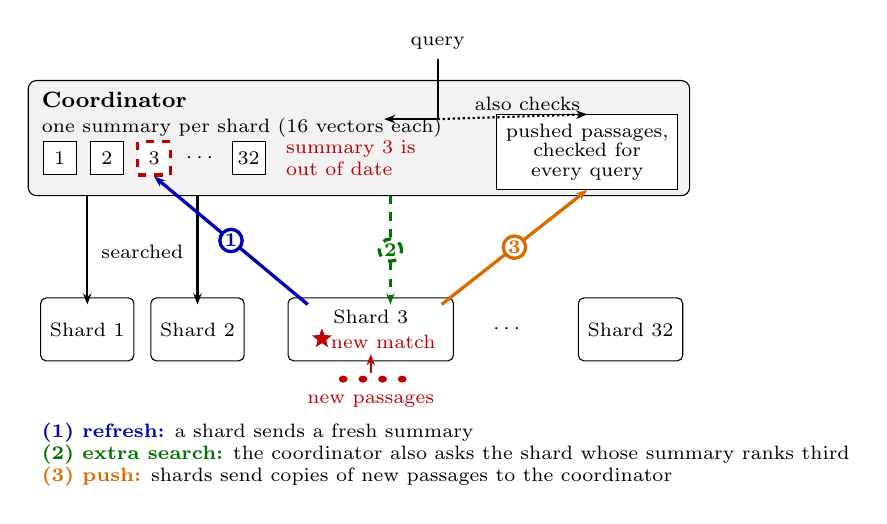
\begin{tikzpicture}[yscale=0.79, font=\scriptsize, >={Stealth[length=4pt]},
  shard/.style={draw, rounded corners=2pt, minimum width=1.15cm, minimum height=0.8cm, fill=white, align=center},
  summ/.style={draw, minimum width=0.42cm, minimum height=0.42cm, inner sep=0pt, fill=white},
  tag/.style={circle, draw, very thick, fill=white, inner sep=0.6pt, font=\scriptsize\bfseries}]
% Coordinator with one summary per shard and a store for pushed passages.
\draw[rounded corners=3pt, fill=black!5] (-4.2,2.15) rectangle (4.2,4.0);
\node[anchor=north west, font=\footnotesize\bfseries] at (-4.15,3.97) {Coordinator};
\node[anchor=north west] at (-4.15,3.55) {one summary per shard (\RNumCentersPerSummary{} vectors each)};
\node[summ] (u1) at (-3.8,2.75) {1};
\node[summ] (u2) at (-3.2,2.75) {2};
\node[summ, draw=red!75!black, dashed, very thick] (u3) at (-2.6,2.75) {3};
\node at (-2.0,2.75) {$\cdots$};
\node[summ] (u32) at (-1.4,2.75) {32};
\node[anchor=west, text=red!75!black, align=left] at (-1.05,2.75) {summary 3 is\\out of date};
\node[draw, fill=white, align=center] (pushed) at (2.9,2.85) {pushed passages,\\[-1pt]checked for\\[-1pt]every query};
% Query: it enters the coordinator, which compares it with the summaries and also checks the pushed passages.
\node[anchor=south] (q) at (1.0,4.35) {query};
\draw[->, thick] (q.south) to (1.0,3.38) to (0.32,3.38);
\draw[->, thick, densely dotted] (1.0,3.38) to node[above, pos=0.6, inner sep=1.5pt] {also checks} (pushed.north);
% Shards.
\node[shard] (s1) at (-3.45,0) {Shard 1};
\node[shard] (s2) at (-2.05,0) {Shard 2};
\node[shard, minimum width=2.1cm] (s3) at (0.15,0) {Shard 3\\[1pt]{\color{red!75!black}\hspace{9pt}new match}};
\node[star, star points=5, star point ratio=2.3, fill=red!75!black, inner sep=1.15pt] at (-0.47,-0.15) {};
\node at (1.9,0) {$\cdots$};
\node[shard] (s32) at (3.45,0) {Shard 32};
% The two searched shards.
\draw[->, thick] (-3.45,2.15) to (-3.45,0.4);
\draw[->, thick] (-2.05,2.15) to (-2.05,0.4);
\node at (-2.75,1.25) {searched};
% New passages arriving at shard 3.
\foreach \x in {-0.2,0.05,0.3,0.55} { \fill[red!75!black] (\x,-0.8) circle (1.6pt); }
\draw[->, red!75!black, thick] (0.15,-0.7) to (0.15,-0.4);
\node[anchor=north, text=red!75!black] at (0.15,-0.9) {new passages};
% The three options: arrows with number tags.
\draw[->, very thick, blue!70!black] (-0.65,0.4) to node[pos=0.5, tag, draw=blue!70!black, text=blue!70!black] {1} (u3.south);
\draw[->, very thick, green!45!black, dashed] (0.4,2.15) to node[pos=0.5, tag, draw=green!45!black, text=green!45!black] {2} (0.4,0.4);
\draw[->, very thick, orange!85!black] (1.05,0.4) to node[pos=0.5, tag, draw=orange!85!black, text=orange!85!black] {3} (pushed.south);
% Key for the three options.
\node[anchor=north west, align=left] at (-4.15,-1.35) {%
{\color{blue!70!black}\textbf{(1) refresh:}} a shard sends a fresh summary\\
{\color{green!45!black}\textbf{(2) extra search:}} the coordinator also asks the shard whose summary ranks third\\
{\color{orange!85!black}\textbf{(3) push:}} shards send copies of new passages to the coordinator};
\end{tikzpicture}

\caption{The problem and the three options. Shard~3 has new passages, but its summary at the coordinator is out of date, so the query can skip shard~3 and miss a new match. Shard~3's summary ranks third closest to the query, so extra search would also ask it.}
\label{fig:problem}
\end{figure}

We study this problem with a simulator, a program that imitates the system one time step at a time.
Each run lasts \RNumNumEpochs{} time steps, and about \RNumSteadyEpochInsertVecs{} new passages arrive per step on average.
In each time step, the coordinator also answers a batch of queries, \RNumPlainQueriesDefault{} by default.
The system may send upkeep messages, paid from a fixed budget of network bytes per time step.
The budget works like a monthly phone data plan without rollover: unused bytes are lost.
We count it in summaries: our default budget of four pays for four summaries per step.
We also test budgets of two and eight.
Even the largest is too small to refresh every shard each step.
So the question is how to spend the budget, and we compare three options (Fig.~\ref{fig:problem}).
The first option is to refresh: some shards send fresh summaries, chosen by a refresh rule.
One such rule, most-changed, picks the shards whose data changed most.
The second is extra search: when the coordinator is unsure which shards to ask, it also asks a third one.
The third is push: shards send copies of their newest passages to the coordinator, which checks them for every query.

We measure accuracy with recall, the share of a query's true best matches that the system returns.
For example, if the system returns seven of ten true best matches, its recall is seven in ten.
Recent recall counts only the best matches that arrived in the last two time steps.
It shows how well the system finds new data, while overall recall counts all best matches, old or new.
When we say that a method wins or is better, we mean that it has higher recent recall.
A difference is clear when our statistical test shows that chance alone would rarely produce it.
A clear lead is fragile when a further check casts doubt on it (Section~\ref{sec:stats}).
Our simulator counts the bytes of every message the budget pays for.
It checks every answer against the exact best matches.

We vary where new passages land: with the most similar shard, all on one shard, or spread over eight shards.
New passages either mix topics the shards already hold or bring new topics, one at a time.
We wrote down our plan and tests before the main analysis; Section~\ref{sec:setup} lists its changes.

When each new passage joins the most similar shard, old summaries often still send queries there.
Refreshing then gains little, and at the default budget and query rate extra search and push beat every refresh rule.
When one shard takes all of a time step's new passages, refresh wins by far on new topics.
On mixed topics, fresh summaries barely help with new matches and slightly lower accuracy overall, so push wins.
When eight shards share the new passages, push wins on mixed topics.
On new topics, refresh has only a fragile lead at a budget of two.
Neither refresh nor push clearly wins at four, and push wins at eight.

Refresh raises a second question: which shards should refresh?
Our sample-query probe, one of five refresh rules, uses practice queries to estimate which fresh summaries would help most.
With eight shards on new topics, it clearly lost to most-changed at budgets of four and eight.
The probe's own messages cost it one summary, but most-changed's small score messages were free.
So we ran a follow-up in which most-changed pays for them, chosen after seeing the main results and so exploratory.
It removed the fragile lead over push.
It also showed that at budgets of four and eight, the probe lost mostly by picking worse shards.
On average, counting each shard's new passages predicted the value of a fresh summary better than the probe did.
We did not try that count as a refresh rule.

\section{Related Work}
\label{sec:related}

% Every sentence that cites or describes a cited work is marked CITE-PLAIN: it rewords the long paper's citing
% sentence (file:line given) without adding a claim. audit/PLAIN_CLAIMS.md gives the verbatim sources/LEDGER.md quote.

Earlier work has studied which items to fetch or refresh first.
% CITE-PLAIN: paper/sections/related.tex:4 (pandey2008crawlorder).
Pandey and Olston \cite{pandey2008crawlorder} first fetch the new web pages that would appear most often in the top results for a set of queries.
% CITE-PLAIN: paper/sections/related.tex:8 (olston2002besteffort, first sentence).
Olston and Widom \cite{olston2002besteffort} study how to keep stored copies as fresh as possible when network capacity is too small for exact copies.
% CITE-PLAIN: paper/sections/related.tex:8 (olston2002besteffort, second sentence).
In their design, each source ranks its own changed items by priority and refreshes those above its own estimate of a shared cutoff.
% Our work (paper/sections/related.tex:14).
Our sample-query probe adapts these ideas to shard summaries, and we compare refreshing with two other uses of the same budget.

Out-of-date summaries also arise in search systems that send each query to only a few document collections.
% CITE-PLAIN: paper/sections/related.tex:6 (ipeirotis2005changes, shokouhi2007updating).
When the collections change, the summaries used to pick them go out of date \cite{ipeirotis2005changes,shokouhi2007updating}.
% CITE-PLAIN: paper/sections/related.tex:6 (shokouhi2007updating).
Shokouhi et al. \cite{shokouhi2007updating} test forty-four changing collections and show that out-of-date collection summaries lower search accuracy.
% CITE-PLAIN: paper/sections/related.tex:6 (shokouhi2007updating, the three policies; query log glossed).
They propose three update policies: update all collections evenly, update more often those that past queries used most, or update by collection size.
% Our work (paper/sections/related.tex:14).
Three of our refresh rules adapt these policies, and we also try two uses of the budget that refresh nothing.

% CITE-PLAIN: paper/sections/related.tex:10 (jose2026repartition, first sentence).
Jose \cite{jose2026repartition} studies when a vector index, a structure that sorts vectors into groups to speed up search, must regroup them as the data changes.
% CITE-PLAIN: paper/sections/related.tex:10 (jose2026repartition, the answer).
The answer depends on how many groups each query searches, and on how much room that leaves to spare.
% CITE-PLAIN: paper/sections/related.tex:10 (jose2026repartition, second sentence).
Slightly outdated group centers, which mark where each group lies, can then be offset by searching a few more groups.
% Our work (paper/sections/related.tex:10 and :14).
That work concerns one index, and our extra search tests a similar trade-off across servers: ask one more shard instead of refreshing summaries.

Finally, some systems spread vector search over many servers.
% CITE-PLAIN: paper/sections/related.tex:12 and system.tex:30 (guo2022manu, segments); hash clause dropped.
Guo et al. \cite{guo2022manu} present Manu, a vector database that writes new data into open blocks called segments.
% CITE-PLAIN: paper/sections/related.tex:12 (guo2022manu, sealing rule).
A segment is closed to new data once it reaches a size limit or sits idle for some time.
% Our work (paper/sections/system.tex:30).
Our one-shard placement, where each time step's new data goes to one shard, loosely models such systems.
% CITE-PLAIN: paper/sections/related.tex:12 (semord2026); synopsis, heartbeat and later clauses dropped.
Wang et al. \cite{semord2026} present Semord, where servers work as equals without a central coordinator.
% CITE-PLAIN: paper/sections/related.tex:12 (semord2026, extra peers); the coordinator-baseline clause dropped.
To make up for queries sent to the wrong servers, Semord's servers contact extra servers, which resembles our extra search.
% Our work (paper/sections/related.tex:12).
We instead study a system with a coordinator whose summaries go out of date under a fixed byte budget.

\section{How the System Works}
\label{sec:system}

\subsection{Data, Shards, and Summaries}

% CITE-PLAIN: paper/sections/setup.tex:36 (nguyen2016msmarco), first part.
We use \RNumCorpusTotalPassages{} passages and \RNumPlainTestQueries{} test queries from the MS MARCO data set \cite{nguyen2016msmarco}.
% CITE-PLAIN: paper/sections/setup.tex:36 (nguyen2016msmarco), second part; "real" and "Bing" dropped.
Its questions come from anonymized user queries, and its passages come from web documents \cite{nguyen2016msmarco}.
% CITE-PLAIN: paper/sections/setup.tex:36 (reimers2019sbert); "six-layer" dropped.
A language model called MiniLM, from the Sentence-Transformers software package \cite{reimers2019sbert}, turns each passage and query into a vector of \RNumVectorDimFloats{} numbers, or \RNumPlainVectorBytes{} bytes.
We compare two vectors by multiplying their matching numbers and adding the products; a higher score means closer meaning.

The $k$-means method sorts vectors into $k$ groups of similar vectors and finds the center, or average point, of each group.
% CITE-PLAIN: paper/sections/system.tex:4 (douze2024faiss); Faiss glossed from the LEDGER quote.
At setup, $k$-means from Faiss, a software package for searching and grouping vectors \cite{douze2024faiss}, splits the starting passages into the \RNumNumShards{} shards.
We call the center of a shard's group its starting center.
Each shard then runs $k$-means with \RNumCentersPerSummary{} groups on its own passages, and its summary is the list of their centers, \RNumSummaryBytes{} bytes.

To answer a query, the coordinator scores each shard by the summary center closest to the query, and it searches the two best-scoring shards.
% CITE-PLAIN: paper/sections/system.tex:4 (malkov2020hnsw); "proximity graph" glossed, the method name dropped.
Each shard stores its vectors in a search graph that links each vector to nearby ones \cite{malkov2020hnsw}.
A search hops along these links toward the query, and it can miss a few close passages.
Each searched shard returns the IDs and scores of the \RNumPlainTopK{} closest passages it finds, and the coordinator keeps the best \RNumPlainTopK{}.
New passages join a shard without moving old ones, and the coordinator keeps the shard's old summary until the shard sends a fresh one.

Each time step draws its queries without repeats from the \RNumPlainTestQueries{} test queries, \RNumPlainQueriesDefault{} by default.
Under starting-center placement, described below, we also test \RNumPlainQueriesLow{} and \RNumPlainQueriesHigh{} queries per time step.

We test two streams, that is, two orders in which new passages arrive.
In the mixed-topic stream, half the passages build the shards, and the other half arrive in random order, \RNumSteadyEpochInsertVecs{} per time step.
In the new-topic stream, we first sort all passages into \RNumPlainTopicClusters{} clusters of similar passages with $k$-means, so each cluster is roughly one topic.
Half of the clusters, picked at random, build the shards.
The other half arrive one cluster after another, about \RNumPlainNewTopicStepVecs{} passages per time step on average, bringing topics the shards have not seen.
% CITE-PLAIN: paper/sections/setup.tex:36 (simhadri2024bigann); "into 64 clusters" dropped.
This design is modeled on the streaming test of the Big-ANN NeurIPS'23 vector-search competition, which inserts points cluster by cluster \cite{simhadri2024bigann}.

Passages never move once stored, and we test three ways to place new ones.
In starting-center placement, each new passage goes to the shard with the closest starting center.
In one-shard placement, all of a time step's new passages go to one shard, and the next time step uses the next shard.
Every refresh rule then refreshes that shard, because rules serve shards with new passages first (Section~\ref{sec:rules}).
In eight-shard placement, a group of eight shards is open in each time step, and the group moves on by eight shards every step.
Each new passage goes to the open shard with the closest starting center, so each step changes five to eight shards.
In these last two placements, the coordinator picks shards only by their summaries and does not know which shards are open.

\begin{table}[!t]
\centering
\caption{What Each Option Sends and What a Budget of 4 Buys per Time Step}
\label{tab:options}
\footnotesize
\setlength{\tabcolsep}{3pt}
\begin{tabular}{@{}l>{\raggedright\arraybackslash}p{4.2cm}r>{\raggedright\arraybackslash}p{1.55cm}@{}}
\toprule
Item & What is sent & Bytes & Budget of 4 buys \\
\midrule
Refresh & One shard's summary (\RNumCentersPerSummary{} centers) & \RNumSummaryBytes{} & \RNumFourRulesSummariesBFour{} summaries \\
Extra search & A query to one more shard, and IDs and scores of its \RNumPlainTopK{} best matches & \RNumPlainSearchBytes{} & Up to \RNumExtraSearchesBFour{} searches \\
Push & A new passage and its ID number & \RNumPlainPushBytes{} & Up to \RNumPushedVecsBFourPerEpoch{} passages \\
\midrule
Probe & Its scores, cutoffs, and counts in one time step (Section~\ref{sec:rules}) & \RNumRNOverheadEpochBytes{} & Room for \RNumRNSummariesBFour{} summaries \\
\bottomrule
\end{tabular}
\end{table}

\subsection{The Budget and Its Three Uses}

The budget counts the network bytes each time step may use, in units of one summary.
We test budgets of two, four, and eight summaries; four is the default and allows \RNumBudgetBFourEpochBytes{} bytes (Table~\ref{tab:options}).
To refresh, a shard rebuilds its summary over all its passages and sends it.
Refreshing all \RNumNumShards{} shards every time step would cost \RNumAlwaysFreshEpochBytes{} bytes, eight times the default budget.

Extra search spends the budget on the queries where the coordinator is least sure.
These are the queries whose second- and third-ranked shards have the closest scores, so either could hold the best matches.
For such a query, the coordinator also searches the third-ranked shard.
The planned version picks these queries after seeing all of the time step's queries, which a system answering each query on arrival could not do.
A budget of four buys up to \RNumExtraSearchesBFour{} extra searches, so at \RNumPlainQueriesLow{} queries per step it also asks a fourth shard for some queries.
The live version decides as each query arrives and asks at most one extra shard per query.
It asks when the score gap is below a cutoff: the gap that would have spent the budget exactly in the previous time step.
With push, shards send up to the budget's worth of their newest passages each time step.
The coordinator keeps them all and checks each query against them.

We also compare against two reference methods that ignore the budget.
Never refresh keeps the first summaries, and refresh all sends all \RNumNumShards{} fresh summaries every time step.
Refresh all is a reference, not the best that refresh can do.
Its rebuilt summaries still have only \RNumCentersPerSummary{} centers, so they describe a shard roughly.
Searching all \RNumNumShards{} shards finds more than \RNumPlainAllShardsMinPct{} of recent matches, so almost all misses come from choosing shards.

\subsection{Five Refresh Rules}
\label{sec:rules}

A refresh rule picks which shards refresh in each time step.
Every rule serves first the shards with new passages since their last refresh, putting any that waited too long ahead.
The waiting limit is twice the time a rule needs to refresh every shard once.
That is \RNumPlainCapBFour{} time steps for a rule that refreshes four summaries per step.
Any budget left over re-sends the summaries of unchanged shards.
Rules that score shards break ties by the lowest shard number.

Rotation lets shards take turns.
Most-searched favors the shards that past test queries were sent to most often, and largest-shard favors the shards with the most passages.
Their scores do not reset after a refresh, so they keep picking the same shards until the waiting limit steps in.
Most-changed scores a shard by the share of its passages that are new.
It multiplies that share by how far the new passages lie, on average, from the nearest center in the shard's last summary.
Each shard computes this score itself, so a real system would send one \RNumScoreBytesPerShard{}-byte score per shard, or \RNumDCScoreEpochBytes{} bytes per time step.
Our main runs did not charge these bytes; the follow-up in Section~\ref{sec:follow} does.

The sample-query probe is our own rule and the most complex.
% CITE-PLAIN: paper/sections/system.tex:61 (pandey2008crawlorder, olston2002besteffort); the two ideas glossed as in Section II.
It adapts two ideas from Section~\ref{sec:related}: ranking by how often items reach top results \cite{pandey2008crawlorder}, and letting each source rank its own changes \cite{olston2002besteffort}.
The probe uses \RNumSampleQueries{} sample queries: practice questions from a separate part of the data set, not the test queries.
The coordinator sends them to every shard once at setup.
Each time step then has three rounds of messages.
First, for each sample query, the coordinator asks the two shards that its summaries rank highest for the scores of their \RNumPlainTopK{} best matches.
Second, it sends every shard two cutoffs for each sample query.
One is the summary score a shard would need to rank in the top two.
The other is the score of the query's \RNumPlainTopK{}th-best match so far.
Third, each shard with new passages rebuilds its summary locally.
For each sample query, it checks whether the rebuilt summary would lift it into the top two.
For those queries, it counts its new passages that score above the \RNumPlainTopK{}th-best cutoff and sends that count.
Among shards with new passages, those over the waiting limit refresh first.
The rest go in order of their counts, with ties going to the lowest shard number.

These rounds cost \RNumRNOverheadEpochBytes{} bytes per time step.
Each budget is a whole number of summaries, and refresh can send only whole summaries.
So any extra charged cost, however small, uses up the room for one summary.
At a budget of four, the probe therefore refreshes three summaries where the other rules refresh four, and its waiting limit is \RNumPlainCapRNBFour{} time steps.

\subsection{Costs We Do Not Count}

The budget pays only for the messages in Table~\ref{tab:options}, and six other costs are left out.
The first is sending new passages to the shards, which is the same for every method.
The second is the probe's setup broadcast of \RNumRNSetupBroadcastBytes{} bytes, its small per-step lists of which sample queries to answer, and its shard work.
Every changed shard rebuilds a summary just to compute its count, and the shards run \RNumRNSampleSearchesPerEpoch{} sample-query searches per time step.
Spread over a run, the broadcast would add \RNumRNSetupAmortEpochBytes{} bytes per step.
That is more than a budget of two, and at four it would leave no room for any summary.
The third is most-changed's score bytes, in the main runs.
The fourth is a free flag that tells the coordinator which shards have new passages.
The flag says only that a shard has new passages, not what they are about.
Every refresh rule uses it to choose shards to refresh, but queries are still sent by summaries alone.
Largest-shard also gets the shard sizes for free.
Charging even a few bytes for this flag would cost every refresh rule one whole summary per time step.
The fifth is the added work of extra search: at the default query rate, shards run \RNumESLoadPctBTwo{} to \RNumESLoadPctBEight{} more searches across budgets.
At a budget of four and \RNumPlainQueriesLow{} queries per step, they run up to \RNumESLoadPctQFifty{} more.
Asking a third shard also means contacting three shards at once or waiting for a second exchange of messages, and neither is counted.
The sixth is push's memory and scanning, up to \RNumPVMaxVecsBFour{} kept passages at a budget of four and \RNumPVMaxVecsBEight{} at eight.
Scanning them for each query takes \RNumPlainPVScanRatioBFour{} to \RNumPlainPVScanRatioBEight{} times as many vector comparisons as scoring all summaries.
Keeping only the last two time steps' \RNumPVFifoVecsBFour{} would give the same recent recall at a budget of four.
Push also assumes the shards know which passages arrived last overall, since it sends the newest ones.
Leaving out the probe's extra costs, most-changed's score bytes, and the free flag favors the refresh rules.
Leaving out the extra search work and push's memory and scanning favors extra search and push.

\section{How We Tested}
\label{sec:setup}

\subsection{Measuring and Comparing Accuracy}
\label{sec:stats}

In every time step, an exact search over all stored passages finds each test query's true \RNumPlainTopK{} best matches and when each was added.
\emph{Recent recall} is the share of a query's true best matches from the current and previous time steps that the system returns.
Only queries with at least one recent match count toward it: about \RNumPlainQueriesWithRecentPctSteady{} of the mixed-topic queries and \RNumPlainQueriesWithRecentPctNewTopic{} of the new-topic queries.
\emph{Overall recall} counts all \RNumPlainTopK{} true best matches, old or new.
We give recall as a percentage and call a difference of one percentage point one \emph{point}.

We run each main setting five times, with seeds numbered \RNumSeedMin{} to \RNumSeedMax{}.
A seed is a number that fixes a run's random choices, the way a recorded shuffle fixes the order of a deck of cards.
It sets the arrival order, the clusters, the queries asked, and the shards' search graphs.
The passages are the same in every run, and all methods see the same queries, so we compare methods query by query.

To compare two methods, we average the difference in recall between them over all queries and seeds.
Other seeds or queries would give a somewhat different average, so we ask how far it could move by chance.
Our main test is a \RNumCIPct{} range found by resampling.
We redraw the five seeds with repeats allowed, like drawing names from a hat and putting each one back.
Within each drawn seed, we redraw its queries the same way.
We recompute the average difference for each of \RNumPlainBootReps{} such redraws, and the middle \RNumCIPct{} of these averages is the range.
If the whole range lies on one side of zero, chance alone would rarely produce the difference, and we call it \emph{clear}.
Otherwise we say there is no clear difference.

Our simpler test uses only the five seed averages of the difference.
Their \emph{spread} is their standard deviation, roughly the typical distance of one seed's average from the mean of all five.
This textbook range is centered on that mean, and its half-width is about \RNumPlainTCritFive{} times the spread divided by the square root of five.
The large factor allows for having only five numbers.
The two tests can disagree because resampling also counts how single queries vary, but with only five seeds it understates how much seeds differ.
So when seeds differ a lot, as in several main eight-shard tests in Table~\ref{tab:main}, our range was \RNumBootNarrowerMin{} to \RNumBootNarrowerMax{} narrower.
When the five seed averages agree closely, the simpler range shrinks and ours can be wider: \RNumBootWiderMThreeRNMinusQLNewTopic{} wider for the probe against most-searched (Section~\ref{sec:res-which}).

A clear lead is \emph{fragile} if it fails any one of four further checks.
Its range must not nearly touch zero, and the simpler test must exclude zero.
No seed may point the other way, and a most-changed lead must survive paying for its score messages (Section~\ref{sec:follow}).

Our ranges treat each asked query as a separate, unrelated sample, although the same \RNumPlainTestQueries{} queries repeat about \RNumQueryRepeatsQTwoHundred{} times per run.
They also rest on the one sample of passages and queries we drew from the data set.
Nor are they widened for our many comparisons, which raises the chance that some clear result is a fluke.
Against other options we use the \emph{best refresh rule}: whichever of the five rules has the highest recent recall in that setting.
Picking it from the same runs we compare favors refresh a little.
This makes the alternatives' tests harder to pass under starting-center placement, and refresh's tests slightly easier under eight-shard placement.

\subsection{Our Plan, Written Before the Main Analysis}

Writing tests down before seeing the results keeps researchers from reporting only the tests that happen to look good.
Before any run, we stored a plan with first settings, message sizes, and three hypotheses, or predictions.
One was that the probe would beat the other rules by at least \RNumPlainGateThreshold{} points under starting-center placement.
A small trial run, or pilot, with one seed (\RNumPilotSeed{}) then showed that refresh gained little there, and all three were replaced.

Before the main runs, a code review and a first written change to the plan, called an addendum, revised the design.
Together they added the new-topic stream, one-shard placement, the three query rates, and an ID number in each pushed passage.
They also replaced a rule that slowly raised waiting shards' scores with a waiting limit set by the budget.
The first addendum set five of the tests below.
Two of them restate pilot results and reuse the pilot's seed, so Section~\ref{sec:res-near} also checks them on the other four seeds.
Testing our analysis program on a partial set of \RNumPartialMOneTestedRuns{} starting-center runs printed one result, which changed no test or rule.
A second addendum came when \RNumPlainAddTwoRunsDone{} of the \RNumPlainAddTwoRunsTotal{} one-shard runs had finished, before anyone looked at them and before any eight-shard run.
It added eight-shard placement, live extra search, and the remaining tests, which is why one-shard runs have only planned extra search.

We call the tests in the plan registered tests; a test that one method beats another passes only if the whole range is above zero.
Under starting-center placement, we tested that refresh all gains less than \RNumPlainGateThreshold{} points on average over never refresh.
We also tested that planned extra search, live extra search, and push each beat the best refresh rule.
Under one-shard placement, we predicted that all five refresh rules match refresh all exactly.
We also tested that refresh beats extra search and push at every budget.
The probe test asked whether the probe beats each other rule by at least \RNumPlainGateThreshold{} points on average, with the whole range above zero.
It ran only if refresh all first gained at least \RNumPlainGateThreshold{} points on average, which we call the \RNumPlainGateThreshold{}-point threshold.
Under one-shard placement, the predicted tie meant that this test could not pass.
Eight-shard placement repeats these tests with live extra search.
It adds a prediction that the four rules other than the probe match refresh all at a budget of eight.

After reading all the main results, we wrote down a follow-up and stored it before running it.
In it, most-changed pays for its score bytes, so it refreshes as many summaries as the probe; we call this version paying most-changed.
Of its \RNumAddThreeTotalRuns{} simulations, \RNumAddThreeMThreeRuns{} used eight-shard placement.
Another \RNumAddThreeMOneRuns{} used starting-center placement at \RNumPlainQueriesHigh{} queries per step.
The last \RNumAddThreeRepRuns{} were reruns with the charge turned off, and they matched the stored main runs on every query.
Because we chose the follow-up after seeing the results, it is exploratory and has no pass or fail tests.
It has \RNumAddThreeTotalIntervals{} ranges, one for each of \RNumAddThreeCompRows{} comparisons on recent and on overall recall, not widened for many comparisons.
Table~\ref{tab:main} shows the eight-shard ones against the probe, push, and live extra search, on recent recall.

The main experiments have \RNumTotalMainRuns{} runs, with none missing, and every run stayed within its budget for the costs we charge.
Runs that ran out of memory were rerun from the same code.
They include some starting-center runs, two eight-shard runs, and \RNumAddThreeMThreeFailedAttempts{} of the \RNumAddThreeMThreeRuns{} eight-shard follow-up runs.

\section{Results}
\label{sec:results}

\begin{table*}[!t]
\centering
\caption{Main Results at \RNumPlainQueriesDefault{} Queries per Time Step: Recent Recall of the First Method Minus the Second, in Points}
\label{tab:main}
\footnotesize
\parbox{\textwidth}{\centering Difference: first method minus second; positive favors the first. Clear winner: the favored method if the \RNumCIPct{} range excludes zero, else neither.}

\vspace{3pt}
\setlength{\tabcolsep}{1.1pt}
\renewcommand{\arraystretch}{0.88}
\begin{tabular}{@{}lclllll@{}}
\toprule
 & & & \multicolumn{2}{l}{Mixed-topic stream} & \multicolumn{2}{l}{New-topic stream} \\
Placement & Budget & First method vs.\ second method & Difference [range] & Clear winner & Difference [range] & Clear winner \\
\midrule
Starting- & 4 & Refresh all vs.\ never refresh & \RNumPlainCellHOneGapSteady{} & Neither & \RNumPlainCellHOneGapNewTopic{} & Refresh all \\
center & 4 & Best refresh rule vs.\ planned extra search & \RNumQSweepRefMinusESQTwoHundredSteadyCell{} & Planned extra search & \RNumQSweepRefMinusESQTwoHundredNewTopicCell{} & Planned extra search \\
 & 4 & Best refresh rule vs.\ live extra search & \RNumQSweepRefMinusESOQTwoHundredSteadyCell{} & Live extra search & \RNumQSweepRefMinusESOQTwoHundredNewTopicCell{} & Live extra search \\
 & 4 & Best refresh rule vs.\ push & \RNumQSweepRefMinusPVQTwoHundredSteadyCell{} & Push & \RNumQSweepRefMinusPVQTwoHundredNewTopicCell{} & Push \\
\midrule
One-shard & 4 & Refresh all vs.\ never refresh & \RNumPlainCellGateMTwoSteady{} & Refresh all & \RNumPlainCellGateMTwoNewTopic{} & Refresh all \\
 & 2 & Any refresh rule vs.\ push & \RNumHFourRefMinusPVBTwoSteadyCell{} & Push & \RNumHFourRefMinusPVBTwoNewTopicCell{} & Refresh \\
 & 4 & Any refresh rule vs.\ push & \RNumHFourRefMinusPVBFourSteadyCell{} & Push & \RNumHFourRefMinusPVBFourNewTopicCell{} & Refresh \\
 & 8 & Any refresh rule vs.\ push & \RNumHFourRefMinusPVBEightSteadyCell{} & Push & \RNumHFourRefMinusPVBEightNewTopicCell{} & Refresh \\
\midrule
Eight- & 4 & Refresh all vs.\ never refresh & \RNumPlainCellGateMThreeSteady{} & Refresh all & \RNumPlainCellGateMThreeNewTopic{} & Refresh all \\
shard & 2 & Best refresh rule vs.\ push & \RNumHFourBRefMinusPVBTwoSteadyCell{} & Push & \RNumHFourBRefMinusPVBTwoNewTopicCell{} & Refresh, fragile \\
 & 4 & Best refresh rule vs.\ push & \RNumHFourBRefMinusPVBFourSteadyCell{} & Push & \RNumHFourBRefMinusPVBFourNewTopicCell{} & Neither \\
 & 8 & Best refresh rule vs.\ push & \RNumHFourBRefMinusPVBEightSteadyCell{} & Push & \RNumHFourBRefMinusPVBEightNewTopicCell{} & Push \\
 & 2 & Best refresh rule vs.\ live extra search & \RNumHFourBRefMinusESOBTwoSteadyCell{} & Live extra search & \RNumHFourBRefMinusESOBTwoNewTopicCell{} & Refresh, fragile \\
 & 4 & Best refresh rule vs.\ live extra search & \RNumHFourBRefMinusESOBFourSteadyCell{} & Live extra search & \RNumHFourBRefMinusESOBFourNewTopicCell{} & Refresh \\
 & 8 & Best refresh rule vs.\ live extra search & \RNumHFourBRefMinusESOBEightSteadyCell{} & Live extra search & \RNumHFourBRefMinusESOBEightNewTopicCell{} & Refresh, fragile \\
 & 4 & Most-changed vs.\ probe & \RNumPlainCellDCMinusRNSteady{} & Neither & \RNumPlainCellDCMinusRNNewTopic{} & Most-changed \\
\midrule
\multicolumn{7}{@{}l}{\emph{Exploratory follow-up (Section~\ref{sec:follow}): most-changed pays for its score bytes, so it refreshes as many summaries as the probe}} \\
Eight- & 2 & Paying most-changed vs.\ probe & \RNumAddThreeXOneRNBTwoSteadyCell{} & Neither & \RNumAddThreeXOneRNBTwoNewTopicCell{} & Neither \\
shard & 4 & Paying most-changed vs.\ probe & \RNumAddThreeXOneRNBFourSteadyCell{} & Neither & \RNumAddThreeXOneRNBFourNewTopicCell{} & Paying most-changed \\
 & 8 & Paying most-changed vs.\ probe & \RNumAddThreeXOneRNBEightSteadyCell{} & Neither & \RNumAddThreeXOneRNBEightNewTopicCell{} & Paying most-changed \\
 & 2 & Paying most-changed vs.\ push & \RNumAddThreeXTwoPVBTwoSteadyCell{} & Push & \RNumAddThreeXTwoPVBTwoNewTopicCell{} & Neither \\
 & 4 & Paying most-changed vs.\ push & \RNumAddThreeXTwoPVBFourSteadyCell{} & Push & \RNumAddThreeXTwoPVBFourNewTopicCell{} & Neither \\
 & 8 & Paying most-changed vs.\ push & \RNumAddThreeXTwoPVBEightSteadyCell{} & Push & \RNumAddThreeXTwoPVBEightNewTopicCell{} & Push \\
 & 2 & Paying most-changed vs.\ live extra search & \RNumAddThreeXTwoESOBTwoSteadyCell{} & Live extra search & \RNumAddThreeXTwoESOBTwoNewTopicCell{} & Neither \\
 & 4 & Paying most-changed vs.\ live extra search & \RNumAddThreeXTwoESOBFourSteadyCell{} & Live extra search & \RNumAddThreeXTwoESOBFourNewTopicCell{} & Refresh \\
 & 8 & Paying most-changed vs.\ live extra search & \RNumAddThreeXTwoESOBEightSteadyCell{} & Live extra search & \RNumAddThreeXTwoESOBEightNewTopicCell{} & Refresh, fragile \\
\bottomrule
\end{tabular}

\vspace{3pt}
\parbox{\textwidth}{\footnotesize Fragile: clear, but failing a further check (Section~\ref{sec:stats}). Best refresh rule: starting-center, the probe on mixed topics and most-changed on new ones; eight-shard, largest-shard at a budget of two on mixed topics, the four tied rules other than the probe at eight, and most-changed otherwise.}
\end{table*}

Table~\ref{tab:main} gives the main differences, and Fig.~\ref{fig:budget} shows recent recall by budget; results use \RNumPlainQueriesDefault{} queries per time step unless we say otherwise.

\subsection{Starting-Center Placement: Old Summaries Often Still Work}
\label{sec:res-near}

When each new passage joins the shard with the closest starting center, the old summaries often already point queries toward the right shard.
So refresh all, at eight times the default budget, raised recent recall by only \RNumPlainHOneSteady{} points on the mixed-topic stream, which is no clear difference.
On the new-topic stream it gained \RNumPlainHOneNewTopic{} points, and the registered test that the gain stays below \RNumPlainGateThreshold{} points passed on both streams.
Even the top ends of both ranges were below it.
Better shard choice could still help a lot.
Suppose each query went to the two shards holding the most of its \RNumPlainTopK{} true best matches, old or new.
On the mixed-topic stream, that finds \RNumPlainOracleMOneSteadyPct{} of recent matches, against \RNumPlainLvlMOneAFSteady{} for refresh all.

At the default budget of four, planned extra search, live extra search, and push each clearly beat every refresh rule on both streams.
Planned extra search and push even beat refresh all, while no refresh rule clearly beat never refresh on the mixed-topic stream.
On each of the four seeds the pilot did not use, planned extra search and push still beat the best refresh rule on both streams.

Extra search helps the coordinator pick good shards in general, not only for new passages.
It also raised overall recall over the best refresh rule by \RNumPlainESOverallMin{} to \RNumPlainESOverallMax{} points.
Push, in contrast, helps only through the new passages it keeps: \RNumMOnePVShareSteady{} of them at a budget of four on the mixed-topic stream.
Never refresh found \RNumPlainLvlMOneNRSteady{} of recent matches there.
If push simply found that same share of the matches never refresh missed, it would reach \RNumPlainMOnePVPredPctSteady{}, and it reached \RNumPlainMOnePVPctSteady{}.
Push raised overall recall over the best refresh rule by only \RNumPlainPVOverallMin{} to \RNumPlainPVOverallMax{} points.

At \RNumPlainQueriesLow{} and \RNumPlainQueriesHigh{} queries per time step, extra search and push still beat every refresh rule on the mixed-topic stream.
On the new-topic stream at \RNumPlainQueriesHigh{} queries, most-changed overtook both versions of extra search.
Its lead was \RNumPlainQSweepESHigh{} to \RNumPlainQSweepESOHigh{} points while its score bytes were free, and it shrinks when they are charged (Section~\ref{sec:follow}).
Push still beat refresh at every query rate.
From \RNumPlainQueriesDefault{} queries up, the planned version of extra search was at most \RNumPlainLookaheadMax{} points ahead of the live one.
At the lowest query rate, it led by \RNumPlainLKQFiftyMin{} to \RNumPlainLKQFiftyMax{} points.
That is partly because the live version asks at most one extra shard per query and spent only about \RNumPlainESOShareQFifty{} of the planned version's bytes.

\begin{figure}[!t]
\centering
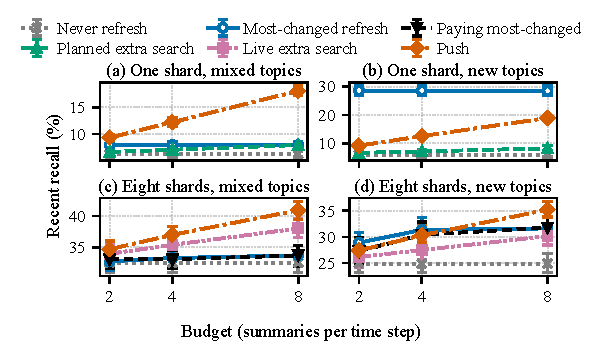
\includegraphics[width=\columnwidth]{figures/fig_budget.pdf}
\caption{Recent recall at each budget, at \RNumPlainQueriesDefault{} queries per time step. Top: one-shard placement, where all refresh rules tie and only planned extra search was run. Bottom: eight-shard placement, with live extra search and paying most-changed (Section~\ref{sec:follow}); most-changed is the best refresh rule there, except that largest-shard is slightly higher at a budget of two on mixed topics. Vertical lines show each method's own \RNumCIPct{} range. Table~\ref{tab:main} compares methods query by query, so it can show a clear difference even where these ranges overlap. Vertical scales differ.}
\label{fig:budget}
\end{figure}

\subsection{One-Shard Placement: The Topics Decide}
\label{sec:res-one}

When one shard takes all of a time step's new passages, all five refresh rules matched refresh all on every query, as predicted.
So the registered probe test could not pass on the new-topic stream.
It was skipped on the mixed-topic stream, where refresh all missed the \RNumPlainGateThreshold{}-point threshold.
Since only one shard changes, the four rules other than the probe spend the rest of each budget re-sending unchanged summaries.
That is \RNumMTwoUnmodShareBTwo{} of a budget of two and \RNumMTwoUnmodShareBEight{} of a budget of eight.

On the mixed-topic stream, never refresh finds \RNumPlainLvlMTwoNRSteady{} of recent matches, about what chance gives when two of \RNumNumShards{} shards are searched.
Refresh all raises this only to \RNumPlainLvlMTwoAFSteady{}, and it lowers overall recall by \RNumPlainGateMTwoOverallSteady{} points, with a drop in every seed.
Plausibly, \RNumCentersPerSummary{} centers cannot describe a shard that holds a mix of every topic.
Push wins at every budget (Fig.~\ref{fig:budget}a), so the registered test that refresh beats both alternatives failed on this stream.
Push keeps \RNumMTwoPVShareBTwo{} to \RNumMTwoPVShareBEight{} of new passages across budgets, and its gain over never refresh closely matches what that share predicts.

On the new-topic stream, the result reverses.
There, each time step's passages come from one or two new clusters, which \RNumCentersPerSummary{} centers describe well.
Refresh all raises recent recall from \RNumPlainLvlMTwoNRNewTopic{} to \RNumPlainLvlMTwoAFNewTopic{}.
Refresh beats push at every budget, but its lead shrinks from \RNumPlainHFourPVBTwoNewTopic{} points at a budget of two to \RNumPlainHFourPVBEightNewTopic{} at eight.
Larger budgets push more passages, while \RNumOneSummary{} fresh summary per time step is already enough.
Refresh also beats planned extra search at every budget, by \RNumPlainHFourESMinNewTopic{} to \RNumPlainHFourESMaxNewTopic{} points, so the registered test passed on this stream.

\subsection{Eight-Shard Placement: Close Calls}
\label{sec:res-eight}

When eight shards share each time step's new passages, more shards change than the smaller budgets can refresh.
On the mixed-topic stream, refresh all again gains little, \RNumPlainGateMThreeSteady{} points, and lowers overall recall by \RNumPlainGateMThreeOverallSteady{} points, with a drop in every seed.
Push beat refresh at every budget, and so did live extra search (Fig.~\ref{fig:budget}c).
On the new-topic stream, refresh all gains \RNumPlainGateMThreeNewTopic{} points and passes the \RNumPlainGateThreshold{}-point threshold on average.
In one seed, though, it gained only \RNumPlainGateMThreeMinSeedGap{} points.
The best two shards per query, chosen as in Section~\ref{sec:res-near}, would find \RNumPlainOracleMThreeSteadyPct{} of recent matches on mixed topics, against \RNumPlainLvlMThreeBFourAFSteady{} for refresh all.
On new topics they would find \RNumPlainOracleMThreeNewTopicPct{}, against \RNumPlainLvlMThreeBFourAFNewTopic{}.

On new topics at a budget of two, most-changed, the best refresh rule, leads push by \RNumPlainHFourBPVBTwoNewTopic{} points, but the lead is fragile.
Its range starts at only \RNumPlainHFourBPVBTwoNewTopicLow{} points, one seed favors push, the simpler test includes zero, and it relies on free score bytes (Section~\ref{sec:follow}).
At a budget of four neither clearly wins, and at eight push wins by \RNumPlainHFourBPVBEightNewTopic{} points (Fig.~\ref{fig:budget}d).
Most-changed also leads live extra search on new topics at every budget, but only the lead at four is not fragile.
At two, one seed favors live extra search and the lead relies on free score bytes; at eight, the simpler test includes zero.
So the registered test that refresh beats both alternatives failed at every budget on mixed topics.
On new topics it passed only at a budget of two, and that pass is fragile.

On overall recall, which also counts older matches, live extra search beat push at every budget, on both streams, by \RNumPlainESOPVOverallMin{} to \RNumPlainESOPVOverallMax{} points.
It also beat refresh there on new topics at budgets of four and eight.

On new topics, push beats never refresh by about \RNumMThreePVNewTopicExcessMin{} to \RNumPlainPVExcessMax{} points more than its share of new passages predicts.
Plausibly, this is because push keeps each time step's last passages, which on this stream tend to come from the newest cluster.
The planned version of extra search was at most \RNumPlainLookaheadMThreeMax{} points ahead of the live one here.
The live version spent slightly less than its budget, as little as \RNumMThreeESOShareOfRefreshBTwoNewTopic{} of it.
That shortfall, worth only about \RNumMThreeESOUnderspendValMin{} to \RNumPlainESOUnderspendMax{} points, changes no winner but blurs how much of the planned lead comes from planning ahead.

\subsection{Which Shards Should Refresh?}
\label{sec:res-which}

We expected the probe to beat each other rule by at least \RNumPlainGateThreshold{} points, but it did not.
In eight-shard placement on new topics at a budget of four, most-changed found \RNumPlainHThreeBRNMinusDCNewTopic{} points more recent matches than the probe (Table~\ref{tab:main}).
The probe showed no clear difference from most-searched or largest-shard.
It clearly beat only rotation, which itself did no better than never refresh at budgets of two and four.
Against most-searched, all five seeds and the simpler test favored the probe, but our range, wider here (Section~\ref{sec:stats}), included zero.
On mixed topics the probe test was skipped, because refresh all missed the \RNumPlainGateThreshold{}-point threshold.
At a budget of eight, the four rules other than the probe refreshed all eight open shards, matching refresh all on every query as predicted.
The probe refreshed seven and on average trailed refresh all by \RNumPlainPredRNBEightNewTopic{} points on new topics.
On mixed topics it trailed by \RNumPlainPredRNBEightSteady{} points, with no clear difference.

The probe's estimate was often zero for every shard.
That happens when no sample query would both move a shard into its top two and find a new passage among its \RNumPlainTopK{} best matches.
In eight-shard placement at a budget of four, this happened in \RNumSpearmanZeroPctNewTopicMThree{} of time steps on new topics and \RNumSpearmanZeroPctSteadyMThree{} on mixed topics.
Under starting-center placement on the mixed-topic stream, its estimate was zero for every shard in \RNumSpearmanZeroPctSteadyMOne{} of time steps.
The probe then falls back to shards over the waiting limit first, then the lowest shard number.

To see which signal points to the shards worth refreshing, we measure each shard's benefit in each time step.
The benefit counts the test queries' true best matches that would move into the two searched shards if that shard alone sent a fresh summary.
It counts old and new matches and does not subtract matches that would drop out.
We rank the \RNumNumShards{} shards by this benefit and by a signal, and compare the two rankings with Spearman's rank correlation.
Like two judges ranking the same contestants, it is one when they agree exactly, near zero when unrelated, and minus one when reversed.
We average it over the time steps in which both the benefit and the probe's estimate differ between shards, and then over the five seeds.
Skipping the steps where the probe cannot tell shards apart favors the probe, and the averages have no ranges.
In eight-shard placement on new topics at a budget of four, the probe's estimate scored \RNumSpearmanRNNewTopicMThree{}, measured on the runs that used the probe.
A plain count of each shard's new passages scored \RNumSpearmanNewVecsNewTopicMThree{}.
Unlike most-changed, the count ignores how far the new passages lie from the old centers, and we did not measure most-changed this way.
On average, the count scored higher in every starting-center and eight-shard setting.
It is free only if the coordinator tracks how many passages each shard receives.

\subsection{Follow-Up: When Most-Changed Pays for Its Scores}
\label{sec:follow}

The follow-up charges most-changed for its own score messages.
Paying \RNumDCScoreEpochBytes{} bytes per time step costs it a whole summary and leaves \RNumAddThreeDCUnspentEpochBytes{} bytes of each step's budget unused.
This is a pessimistic case for most-changed, because unused bytes do not carry over, and we did not run a version where they do.
If unused bytes carried over, its \RNumDCScoreEpochBytes{} bytes per step would add up to less than one summary over a \RNumNumEpochs{}-step run.

Paying most-changed refreshes as many summaries as the probe, so comparing the two shows which picks better shards.
Of most-changed's \RNumPlainHThreeBRNMinusDCNewTopic{}-point lead over the probe in the main runs, at a budget of four on new topics, \RNumPlainXOneRNBFourNewTopic{} points remained.
The other \RNumPlainXThreeDCBFourNewTopic{} points came from the summary that the probe's messages cost it.
At a budget of eight, paying most-changed led by \RNumPlainXOneRNBEightNewTopic{} points.
All \RNumAddThreeXOnePosSeedsBFourBEight{} seed results at these two budgets favored it.
At a budget of two on new topics, \RNumPlainXThreeDCBTwoNewTopic{} of the probe's \RNumPlainRNLossBTwoNewTopic{}-point main-run loss came from the lost summary.
That part is fragile, because the simpler test includes zero.
At that budget, and on mixed topics, the two rules showed no clear difference.
This comparison still favors the probe, which sends \RNumAddThreeRNExtraEpochBytesVsChargedDC{} more bytes per time step and keeps its setup broadcast free.
At a budget of four on new topics, paying most-changed led by \RNumPlainXOneAllZeroGap{} points in steps where the probe's estimate was all zero.
In the other steps it led by \RNumPlainXOneNonZeroGap{}.
There, the waiting limit forced \RNumAddThreeRNForcedSumBFourNewTopic{} of the probe's \RNumAddThreeTotalRefreshesBFour{} refreshes.
It forced \RNumAddThreeChargedDCForcedSumBFourNewTopic{} of the \RNumAddThreeTotalRefreshesBFour{} made by paying most-changed.

Against push on new topics, paying most-changed lost the fragile lead that most-changed had at a budget of two.
Push was then \RNumPlainXTwoPVBTwoNewTopic{} points ahead, with no clear difference, so this is not a win for push either.
At a budget of four there was still no clear winner, and at eight push led by \RNumPlainXTwoPVBEightNewTopic{} points.
Against live extra search on new topics, paying most-changed had no clear lead at a budget of two and a clear lead at four.
At eight its lead was fragile, because one seed pointed the other way.
On overall recall, live extra search led it on new topics at budgets of four and eight, though at four the simpler test includes zero.
On mixed topics, push and live extra search each led paying most-changed at every budget.
At a budget of eight, paying most-changed refreshes seven summaries, so it no longer matches refresh all on every query.
On new topics it differs from unpaid most-changed by only \RNumPlainXThreeDCBEightNewTopic{} points, with no clear difference.

The follow-up also reran starting-center placement at \RNumPlainQueriesHigh{} queries per step, where most-changed had overtaken extra search on new topics.
Paying most-changed still edged planned extra search there, by only \RNumPlainXFourESNewTopic{} points.
That lead is fragile: its range barely clears zero, and it touches zero when we redo the resampling with other random draws.
It also comes only from the first \RNumPlainXFourEarlySteps{} of the \RNumNumEpochs{} time steps.
Planned extra search was \RNumPlainXFourLateGap{} points ahead in later steps and \RNumPlainXFourOverallGap{} ahead on overall recall, with no clear difference there.
Paying most-changed also led live extra search by \RNumPlainXFourESONewTopic{} points, with a range starting at \RNumPlainXFourESONewTopicLow{}.
Push still beats paying most-changed there, by \RNumPlainXFourPVNewTopic{} points.

\section{Limits and What We Did Not Test}
\label{sec:limits}

Our simulator runs as a single program, so all shards share one machine.
It does not model network delays, waiting in queues, work done at the same time, or failures.
All runs use one data set and one text model, with \RNumCorpusTotalPassages{} passages drawn once with a fixed seed.
They also use five seeds and fixed sizes: \RNumNumShards{} shards, two searched shards per query, and \RNumCentersPerSummary{} centers per summary.

About \RNumSteadyEpochInsertVecs{} passages arrive per time step, and a summary stays the same size as arrivals grow.
But the share of new passages that push can keep at a fixed budget falls, so higher arrival rates may favor refresh.
In one-shard and eight-shard placement, new passages join shards that keep their starting passages, and a fresh summary covers the whole shard.
On mixed topics this lowered overall recall, plausibly because the centers shift toward the random new passages.
Separate summaries for new data might avoid this, but we did not model them.
A coordinator that knows which shards are open could also reach them without upkeep traffic.
Saving re-sent summary bytes, carrying unused bytes over, and a refresh rule based on the plain count are also untested.

\section{Conclusion}
\label{sec:conclusion}

When shard summaries go out of date, a split vector database can miss new matches.
The best use of a fixed network budget for finding them depends on where new data goes and its topics.

In our tested setting, the results suggest three rules of thumb.
First, when new data joins the most similar shard, spend the budget on extra search if shards have spare capacity.
Push is the other choice, if the coordinator can store and scan new passages.
Extra search won at every query rate on mixed topics and up to \RNumPlainQueriesDefault{} queries per step on new topics.
At \RNumPlainQueriesHigh{} queries on new topics, most-changed overtook it, but only fragilely once it paid for its scores.
Push won at every rate we tried, but at the default rate extra search raised overall recall far more.
Second, when each step's new data lands on one shard, refresh that shard if the data brings a new topic.
When topics are mixed, push instead, since fresh summaries there also lower overall recall.
When eight shards share the new data, push on mixed topics.
On a new topic, neither refresh nor push wins reliably at the smaller budgets, and push wins at the largest.
Third, to choose which shards to refresh, rank them by how much their data changed rather than by probing.
Our evidence comes from eight shards on new topics at budgets of four and eight, even with scores paid.
It also rests on recall alone, since we did not score most-changed with our ranking measure.

These results come from one simulator and one data set, with some costs uncharged.
Future work should test summaries that adapt to new data and coordinators that know where new data goes.
It should also test higher arrival rates and slow responses.


\section*{Acknowledgment}
Gemini (Google) drafted the simulator, analysis code, and number scripts, and an earlier draft of the text.
Claude (Anthropic) rewrote that draft into this version, wrote the figure code, added scripted number commands, checked each
citation against its source, and recomputed reported numbers. Gemini, Claude, and Codex (OpenAI) reviewed drafts;
Codex edited no files. Result numbers come from scripts run on stored run outputs. \ifanonymous The authors take\else The author takes\fi{} responsibility
for the content.

\bibliographystyle{IEEEtran}
\bibliography{bstctl,refs}

\end{document}
